\documentclass{article}

%in that file you will find the packages and other macro needed like \R for the
%real number set.
\usepackage{vmargin}
\setmarginsrb{28mm}{25mm}{28mm}{25mm}{0pt}{0mm}{0pt}{0mm}
\setlength{\footskip}{20pt}
\usepackage{amssymb}
\usepackage{amsmath}
\usepackage{amsthm}
\usepackage{pgfplots}
\pgfplotsset{compat=1.9} % for backward compatibility
\usepackage{graphicx}
\usepackage[utf8]{inputenc}
\usepackage{tikz}
\usepackage{bbm}
\usepackage{subcaption}
% \usepackage[boxruled]{algorithm2e}
\usepackage{algpseudocode}
\usepackage{algorithm}
\usetikzlibrary{positioning}
\usepackage{caption}
\usepackage{mathtools}
\usepackage{lipsum}
\usepackage[title,titletoc]{appendix}
\usepackage{booktabs}
\usepackage{here}
%Literatur
\usepackage[%
    backend=biber,
    sortcites, % sort automatically
    sorting=nty, % sort order
    safeinputenc, % solves problems with unicode-formatted author names etc.
    citestyle=alphabetic, %
    bibstyle=alphabetic, %
    hyperref=true, % provide clickable links
    maxbibnames=3, % shorten author list for more than 3 names
    maxcitenames=3, % use at most 3 names for key
    url=false, % do not print URLs
    doi=false, % do not print DOIs
    giveninits=true,
    ]%
{biblatex}
% automatische Anführungszeichen
\usepackage[autostyle=true]{csquotes}
\usepackage[hidelinks]{hyperref}
%some weird packages
\usepackage{halloweenmath}
\usepackage{txfonts}
\usepackage{knitting}
\usepackage{listings}
\usepackage{xcolor}
\usepackage{multirow}
\usepackage{wrapfig}

\definecolor{codegreen}{rgb}{0,0.4,0}
\definecolor{codegray}{rgb}{0.5,0.5,0.5}
\definecolor{mymauve}{rgb}{0.58,0,0.82}
\definecolor{codepurple}{rgb}{0.58,0,0.82}
\definecolor{backcolour}{rgb}{0.95,0.95,0.92}

\lstdefinestyle{mystyle}{
    %backgroundcolor=\color{backcolour},
    commentstyle=\color{codegreen},
    keywordstyle=\color{mymauve},
    numberstyle=\tiny\color{codegray},
    stringstyle=\color{codepurple},
    basicstyle=\ttfamily\footnotesize,
    breakatwhitespace=false,
    breaklines=true,
    captionpos=b,
    keepspaces=true,
    numbers=left,
    numbersep=5pt,
    showspaces=false,
    showstringspaces=false,
    showtabs=false,
    tabsize=2
}

\lstset{style=mystyle}

\DeclarePairedDelimiter{\ceil}{\lceil}{\rceil}
\renewcommand{\phi}{\varphi}
\newcommand{\eqtext}[1]{\ensuremath{\stackrel{#1}{=}}}
\newcommand{\leqtext}[1]{\ensuremath{\stackrel{#1}{\leq}}}
\newtheorem{theorem}{Proposition}[section]
\newtheorem{lemma}{Lemma}[section]
\newtheorem{remark}{Remark}[section]
\newcommand{\N}{\mathbb{N}}
\newcommand{\R}{\mathbb{R}}
\newcommand{\E}{\mathbb{E}}
\newcommand{\epl}{\varepsilon}

\renewcommand{\algorithmicrequire}{\textbf{Input:}}
\renewcommand{\algorithmicensure}{\textbf{Output:}}

\theoremstyle{definition}
\newtheorem{definition}{Definition}[section]

\addbibresource{Project2.bib}

\date{\today}

\begin{document}

%this creates the title page. You must complete the information there
\hypersetup{pageanchor=false}
\begin{titlepage}
\newcommand{\HRule}{\rule{\linewidth}{0.5mm}} % Defines a new command for the horizontal lines, change thickness here

\center % Center everything on the page

%----------------------------------------------------------------------------------------
%   HEADING SECTIONS
%----------------------------------------------------------------------------------------

\vspace{3cm}
\textsc{\LARGE École polytechnique fédérale de Lausanne}\\[1.5cm] % Name of your university/college
\textsc{\Large HPC for Numerical Methods and Data Analysis}\\[0.5cm] % Major heading such as course name
\textsc{\large Course Project Fall 2023}\\[0.5cm] % Minor heading such as course title

%----------------------------------------------------------------------------------------
%   TITLE SECTION
%----------------------------------------------------------------------------------------

\HRule \\[0.4cm] % line above and under the title
{ \huge \bfseries Randomized Nyström Low-Rank Approximation}\\[0.4cm] % Title of your document
\HRule \\[1.5cm]

%----------------------------------------------------------------------------------------
%   AUTHOR SECTION
%----------------------------------------------------------------------------------------

\begin{minipage}{0.4\textwidth}
\begin{flushleft} \large
\emph{Authors:}\\
Christian \textsc{Mikkelstrup}\\
Julian Philipp \textsc{Schmitt} % Your name
\end{flushleft}
\end{minipage}
~
\begin{minipage}{0.4\textwidth}
\begin{flushright} \large
\emph{Supervisor:} \\
Prof. Laura \textsc{Grigori} % Supervisor's Name
\end{flushright}
\end{minipage}\\[10cm]

%----------------------------------------------------------------------------------------
%   LOGO SECTION
%----------------------------------------------------------------------------------------


\includegraphics[width=0.4\linewidth]{Logo}\\[1cm] % Include a department/university logo - this will require the graphicx package

%----------------------------------------------------------------------------------------

\vfill % Fill the rest of the page with whitespace

\end{titlepage}


\clearpage
\thispagestyle{empty}
\tableofcontents

\clearpage
\hypersetup{pageanchor=true} % to start numbering after title and ToC pages
\pagenumbering{arabic}
\setcounter{page}{1}

\section{Introduction}
In this project, we study the randomized Nyström approximation algorithm for the
low-rank approximation of a positive-semidefinite matrix $A\in \mathbb{R}^{n
\times n}$. There are several important applications for this theory, such as
image processing, PCA, or solving integral equations. However, the most common
practical setting are kernel methods for large-scale machine-learning problems.
Since these algorithms scale at least quadratic in the number of data points,
low-rank approximations are essential to obtain reasonable storage usage and
computational costs.\newline

The randomized Nyström approximation is based on a random sketching matrix
$\Omega \in \mathbb{R}^{n \times l}$ and the formula:
\begin{align}
    \label{nyst:sketching_formula}
    A_{Nyst} = (A \Omega) (\Omega^T A \Omega)^\dagger (\Omega^T A)
\end{align}
where $l \ll n$ is the sketching dimension and $(\Omega^T A \Omega)^\dagger$
denotes the pseudo-inverse. In particular, the algorithm we used computes a
fixed-rank $k \leq l$ approximation by truncating the sketched matrix
$A_{Nyst}$. Our goal is to efficiently parallelize this alogrithm. Key aspects
of our investigations are numerical stability, scalability, performance (in
terms of runtime), and the approximation of the leading $k$ singular values of
$A$.\newline

\section{Randomized Nyström Algorithm}\label{sec:rand_nystrom_alg}

We start by describing the efficient computation of a rank-k approximation from
the sketching formula (\ref{nyst:sketching_formula}). We obtain such an
approximation by simply truncating the \textit{singular value decomposition}
(SVD) of $A_{Nyst}$, as this leads to the best rank-k approximation of
\eqref{nyst:sketching_formula} \cite{tropp2017fixedrank}. In the following, we
denote this truncation by $[\![A_{Nyst}]\!]_k$ and note that this method is also
called \textit{modified fixed-rank Nyström via $QR$} in literature.\newline

The \enquote{naive} approach of computing $A_{Nyst}$ and afterwards the
corresponding truncated SVD would be computationally heavy because calculating
the SVD of large matrices is very expensive. Algorithm \ref{algo:nyström}
illustrates an alternative which directly computes $[\![A_{Nyst}]\!]_k$ by
decomposing $A_{Nyst}$. First, we calculate the two sketched matrices $C = A
\Omega \in \mathbb{R}^{n \times l}$ as well as $B = \Omega^T A \Omega \in
\mathbb{R}^{l \times l}$. This is the part of the algorithm with the highest
computational cost since it consists of two high-dimensional matrix-matrix
products. Nevertheless, in the next section we will present some sketching
techniques which lower these costs. Next, we factorize $B = LL^T$, e.g. using
the Cholesky decomposition, and $Z = C L^{-T} = QR \in \mathbb{R}^{n \times l}$
via the $QR$ decomposition. This leads to
\begin{align*}
    [\![A_{Nyst}]\!]_k
    &= [\![(A \Omega) (\Omega^T A \Omega)^\dagger (\Omega^T A)]\!]_k\\
    &= [\![CL^{-T}L^{-1}C^T]\!]_k = [\![ZZ^T]\!]_k \\
    &= [\![QRR^TQ^T]\!]_k = QU_k\Sigma_k V_k^T V_k \Sigma_k^T U_k^TQ^T\\
    &= QU_k\Sigma_k \Sigma_k U_k^TQ^T = QU_k\Sigma_k^2 U_k^TQ^T
\end{align*}
where $U_k \Sigma_k V_k^T$ is the truncated SVD of $R \in \mathbb{R}^{l \times
l}$. Recall $l \ll n$ and note that the SVD is only calculated on an $l \times
l$ matrix providing significantly lower runtimes. Moreover, in our Python
implementation (for details see Section \ref{sec:num_stability}) we do not
calculate the entire SVD and throw away the rows and columns we do not need, but
instead compute the partial SVD, extracting only the $k$ singular values of the
largest magnitude \cite{scipy_svds}. This approach provides further speedup for
low approximation ranks.\newline

Note that in step 7 of Algorithm \ref{algo:nyström}, instead of computing
$\hat{U}_k$ as $Q U_k$ we could use $\hat{U}_k = Z V_k \Sigma_k^{-1}$, which
would provide less numerical stability but entail a smaller computational cost.
This smaller computational cost comes because one could omit the computation of
the $Q$-factor of the $QR$ decomposition. However, in practice, we observed that
computing $\hat{U}_k$ as $Z V_k \Sigma_k^{-1}$ reduces the runtime of our
algorithm by not more than 10\%. One reason for this might be that we worked
with $n=2^{13}$ and accordingly $Z \in \mathbb{R}^{8192 \times l}$ is still
relatively small. For larger dimensions, it could be worth it to consider
$\hat{U}_k = Z V_k \Sigma_k^{-1}$, but we decided to focus on $\hat{U}_k = Q
U_k$ in this report.\newline

Moreover, it is important to mention that the matrix $B = \Omega^T A \Omega$ can
be rank-deficient, e.g. if the rank of $A$ or $\Omega$ is smaller than $l$. In
this case, it is not possible to obtain the Cholesky factorization in step 3.
Instead, one can use the square root of $\Omega^T A \Omega$ computed via the SVD
or eigendecomposition: Let $B = U \Sigma V^T$ be the SVD of $B$. Since $B$ is
symmetric and non-negative definite, it holds $V = U$. We simply set $L = U
\sqrt{\Sigma} V^T$ and obtain $LL^T = U \sqrt{\Sigma} V^T V \sqrt{\Sigma} U^T =
U \Sigma U^T = U \Sigma V^T = B$. Note that the SVD based approach is
accompanied by considerably higher computational costs compared to the Cholesky
decomposition. Not only is it more expensive to calculate the SVD, but
additionally the matrix product $L = U \sqrt{\Sigma} V^T$ must be determined.
Further, when using the Cholesky decomposition, one can exploit the fact that
$L$ is triangular and calculate $Z = C L^{-T}$ via backward substitution which
implies\footnote{'$\dot{=}$' indicates equality when omitting lower-order terms}
\# flops $\dot{=}\ l^2$. In contrast, when using the SVD one has to solve a
general linear system which does not perform better than $O(l^3)$. Although
there are alternatives, e.g. making $A$ full-rank by shifting
\cite{tropp2017fixedrank}, we will stick to the SVD approach.\newline

Finally, we remark that Algorithm \ref{algo:nyström} is a is a
\textit{streaming} algorithm since it requires only one pass over the data or
$A$, respectively. This is a major advantage compared to e.g. the randomized
singular value decomposition.
\begin{algorithm}[t]
    \caption{Randomized Nyström} \label{algo:nyström}
    \begin{algorithmic}[1]
        \Require $A \in \mathbb{R}^{n \times n}, \Omega \in
                    \mathbb{R}^{n \times l}$
        \State $C = A \Omega \in \mathbb{R}^{n \times l}$
        \State $B = \Omega^T C \in \mathbb{R}^{l \times l}$
        \State $B = LL^T$ (via Cholesky)
        \State $Z = C L^{-T}$ (via substitution on triangular system)
        \State $Z = QR$ ($QR$ decomposition)
        \State Compute rank-k SVD of $R$: $U_k \Sigma_k V_k^T$
        \State $\hat{U}_k = Q U_k$
        \Ensure $\llbracket A_{Nyst}\rrbracket_k = \hat{U}_k \Sigma_k^2
                \hat{U}_k^T$
    \end{algorithmic}
\end{algorithm}

\subsection{Sketching Techniques}
In this section, we describe the construction of the sketching matrix $\Omega
\in \mathbb{R}^{n \times l}$. In particular, we are concerned with randomized
methods for dimension reduction and it is therefore useful to define the
so-called \textit{oblivious $l_2$-subspace embedding} (OSE):
\begin{definition}[OSE]
    Let $0 < \epsilon < 1$ and $0 < \delta < 1$. A random matrix $\Omega \in
    \mathbb{R}^{n \times l}$ is a $(\epsilon, \delta, d)$ OSE, if for any fixed
    $d$-dimensional subspace $V \subseteq \mathbb{R}^{n}$,
    \begin{align*}
        \left| ||x||_2^2 - ||\Omega^T x||_2^2 \right| \leq \epsilon \cdot ||x||_2^2
        \quad \forall x \in V
    \end{align*}
    holds with probability $1 - \delta$.
\end{definition}

For the randomized Nyström approximation, we considered two different sketching
techniques: the \textit{block Subsampled Randomized Hadamard Transform} (BSRHT)
\cite{balabanov2022} and a \textit{Short-Axis-Sparse Sketching Operator} (SASO)
\cite{murray2023}. Both are structured random matrices which aim to reduce the
computational costs of the matrix-matrix product $A \Omega$.\newline

The BSRHT is a version of the Subsampled Randomized Hadamard Transform (SRHT)
specifically designed for distributed architectures. For $n$ being a power of
two, the SRHT can be defined as
\begin{align*}
    \Omega^T = \sqrt{\frac{n}{l}} R H D,
\end{align*}
where
\begin{itemize}
    \item $H\in \mathbb{R}^{n \times n}$ is the normalized Walsh–Hadamard matrix
            which is defined recursively as:
    \begin{align*}
        H_2 = \begin{pmatrix}
            1 & 1 \\
            1 & -1
        \end{pmatrix},
        \qquad
        H_n = \begin{pmatrix}
            H_{n/2} & H_{n/2}\\
            H_{n/2} & -H_{n/2}
        \end{pmatrix}
        \qquad \text{and} \qquad
        H = n^{-1/2} H_n
    \end{align*}
    \item $D\in \mathbb{R}^{n \times n}$ is a diagonal matrix with i.i.d. random
            variables $\sim$ Uniform$(\{\pm 1\})$.
    \item $R\in \mathbb{R}^{n \times l}$ is a subset of $l$ randomly sampled
            rows from the $n \times n$ identity matrix.
\end{itemize}
Note that we can always zero-pad the data to ensure that $n$ is a power of 2.
Now, for $P$ different processors, the BSRHT can be constructed block-wise from
the SRHT as:
\begin{align}
    \label{BRSHT}
    \Omega^T
    = \begin{pmatrix}
        \Omega_1^T & \ldots & \Omega_P^T
    \end{pmatrix}
    = \sqrt{\frac{n}{Pl}}
    \begin{pmatrix}
        D_{L1} & \ldots & D_{LP}
    \end{pmatrix}
    \begin{pmatrix}
        RH \\
        & \ddots \\
        && RH
    \end{pmatrix}
    \begin{pmatrix}
        D_{R1}\\
        & \ddots \\
        && D_{RP}
    \end{pmatrix}
\end{align}
with
\begin{itemize}
    \item $H\in \mathbb{R}^{n/P \times n/P}$ being the normalized Walsh–Hadamard
            matrix.
    \item $D_{L i}\in \mathbb{R}^{l \times l}, D_{R i}\in \mathbb{R}^{n/P \times
            n/P}$ being diagonal matrices with i.i.d. Rademacher entries $\pm
            1$.
    \item $R\in \mathbb{R}^{l \times n/P}$ being a  uniform sampling matrix,
            sampling along the rows.
\end{itemize}
The main advantage of the BRSHT compared to the SRHT is that the matrix-matrix
product distributed across $P$ processors with row-wise partitioning can be
computed as $A\Omega = \sum_{i=1}^P A_i \Omega_i$. In particular, one can
compute the local contributions $A_i \Omega_i$ independently on each processor
and finally sum-reduce them. Since $\Omega$ is distributed across processors, we
never have to produce the large concatenated matrices in \eqref{BRSHT}, as we
can calculate $\Omega_i=\sqrt{\frac{n}{Pl}} D_{Li} R H D_{Ri}$. Furthermore, we
can utilize that $D_{Li}$ and $D_{Ri}$ are diagonal matrices, and that $R$
simply samples rows, such that only $H$ has to be explicitly created and
modified to get $\Omega_i$. Also note that because the same $R$ has to be
generated on each processor, the root processor has to broadcast a seed for
generating this sampling matrix. We chose to sample rows without replacement,
but the other case is discussed in \cite{balabanov2022}. Moreover, we remark
that one can exploit the Fast-Johnson-Lindenstrauß transform to reduce the flops
required for applying BRSHT \cite{balabanov2022}. However, this requires a
special implementation that we do not consider here. \citeauthor{balabanov2022}
\cite{balabanov2022} showed that the construction of $\Omega$ as in
(\ref{BRSHT}) yields an $(\epsilon, \delta, d)$ \textit{oblivious subspace
embedding} (OSE) if
\begin{align}
    \label{BRSHT:OSE_Condition}
    n \geq l \geq 3.7 \epsilon^{-2}
    \left(
        \sqrt{d} + 4 \sqrt{\log \frac{n}{\delta} + 6.3}
    \right)^2
    \log \frac{5d}{\delta}
\end{align}
with $0 < \epsilon < 1$ and $0 < \delta < 1$. This implies compatability with
all randomized methods that rely on OSEs and in particular with the Nyström
approximation. Note that condition (\ref{BRSHT:OSE_Condition}) can be used to
choose a proper sketching dimension $l$.\newline

For the construction of the SASO, we call the rows of $\Omega$
\textit{short-axis vectors} since $l \ll n$. These short-axis vectors should be
independent of one another and have a small, fixed number of non-zero elements.
In general, there are different ways of selecting the locations of the non-zero
elements. We decided to sample $k'$ indices uniformly from $1$ to $l$ without
replacement, once for each row. Furthermore, the values of the non-zeros are
drawn independently and uniformly from $[-2,-1] \cup [1, 2]$. Compared to i.i.d.
Rademachers this can protect against the possibility of a given column of
$\Omega$ being orthogonal to a row of $A$ \cite{murray2023}. Finally, we set $k'
= \min\{8, l\}$ following experimental results mentioned in \cite{murray2023}.
In theory, the SASO is a faster sketching operator than BRSHT because of its
high sparsity. However, to exploit this one would have to implement the
corresponding algorithm using sparse vectors (implementation notes are available
in \cite{murray2023}). We did not do so and therefore we expect that that SASO
and BRSHT will perform similar w.r.t. the runtime. Last, there are theoretical
sketching guaranties for SASO, but these are not as strong as
(\ref{BRSHT:OSE_Condition}) for BRSHT and one might expect that SRHT (and BRSHT)
provide better results in terms of numerical stability. Nevertheless, we did not
observe this effect in our experiments (see Section \ref{sec:num_stability})
which might be due to the fact that we did not use simple Rademachers as
non-zero elements for SASO.

\section{Parallelization of the Nyström Algorithm}\label{sec:parallel_nystrom}
Having seen the (sequential) randomized Nyström approximation in Algorithm
\ref{algo:nyström}, we focus now on the corresponding parallelization for a
distributed system. For $A \in \mathbb{R}^{n \times n}$ and $\Omega \in
\mathbb{R}^{n \times l}$, the Nyström approximation can be divided into 4 steps:
\begin{enumerate}
    \item Sketching: $C = A \Omega \in \mathbb{R}^{n \times l}, B = \Omega^T C
            \in \mathbb{R}^{l \times l}$
    \item Decomposition: $B = LL^T$ (e.g. via Cholesky) with $L \in
            \mathbb{R}^{l \times l}$ and $Z = C L^{-T} \in \mathbb{R}^{n \times
            l}$
    \item $QR$ factorization: $Z = QR$ with $Q \in \mathbb{R}^{n \times l}$ and
            $R \in \mathbb{R}^{l \times l}$
    \item Rank-k SVD of $R$: $U_k \Sigma_k V_k^T$ and $\hat{U}_k = Q U_k$
\end{enumerate}
Considering $l \ll n$, we aim to parallelize the sketching of $A$ and use the
TSQR algorithm for the $QR$ factorization of the tall-skinny matrix $Z$. The
decomposition of $B$ and the SVD of $R$ can be computed sequentially since both
matrices are small (dimensions only dependent on $l$).\newline

For the parallel sketching, we work with a 2D block distribution of $A$ and a
row-block distribution of $\Omega$. From now on, we assume that the number of
processors $P$ is a power of 4 because we need $\sqrt{P}$ to be an integer for
the 2D distribution and later we will need a power of 2 for TSQR. For $P=4$, the
matrix partitioning is the following:
\begin{align*}
    C = A \Omega
    = \begin{pmatrix}
        A_{11} & A_{12} \\
        A_{21} & A_{22}
    \end{pmatrix}
    \begin{pmatrix}
        \Omega_1 \\
        \Omega_2
    \end{pmatrix}
    &= \begin{pmatrix}
        A_{11} \Omega_1 + A_{12} \Omega_2 \\
        A_{21} \Omega_1 + A_{22} \Omega_2
    \end{pmatrix}
    \\
    B = \Omega^T C
    = \begin{pmatrix}
        \Omega_1^T & \Omega_2^T
    \end{pmatrix}
    \begin{pmatrix}
        C_1 \\
        C_2
    \end{pmatrix}
    &= \begin{pmatrix}
        \Omega_1^T & \Omega_2^T
    \end{pmatrix}
    \begin{pmatrix}
        A_{11} \Omega_1 + A_{12} \Omega_2 \\
        A_{21} \Omega_1 + A_{22} \Omega_2
    \end{pmatrix}
\end{align*}

\begin{algorithm}[t]
    \caption{Parallel Sketching} \label{algo:sketching}
    \begin{algorithmic}[1]
        \Require $A \in \mathbb{R}^{n \times n}, \Omega \in
                    \mathbb{R}^{n \times l}$
        \State Root processor: broadcast information for generating blocks of
                $\Omega$
        \For{\text{all processors $P_{ij}$ with $i,j = 1:\sqrt{P}$ in parallel}}
            \State Generate block $\Omega_j$
            \State Compute $C_{ij} = A_{ij} \Omega_j$
            \State Sum-Reduce among rows $C_i = \sum_{j = 1}^{\sqrt{P}} C_{ij}$
                    with root being $P_{ii}$
            \State Scatter $C_i$ into $C_{ki}$ among processors in same column
            \State Compute $B_{ki} = \Omega_j[(k-1) n/P : k n/P, :]^T \ C_{ki}$
        \EndFor
        \State Sum-Reduce $B = \sum_{k,i = 1}^{\sqrt{P}, \sqrt{P}} B_{ki}$
        \Ensure $B, C$
    \end{algorithmic}
\end{algorithm}

\begin{wrapfigure}[51]{TR}{0.4\textwidth}
\centering
\begin{subfigure}[t]{\dimexpr0.35\textwidth+20pt\relax}
    \makebox[20pt]{\raisebox{65pt}{\rotatebox[origin=c]{90}{MNIST}}}%
    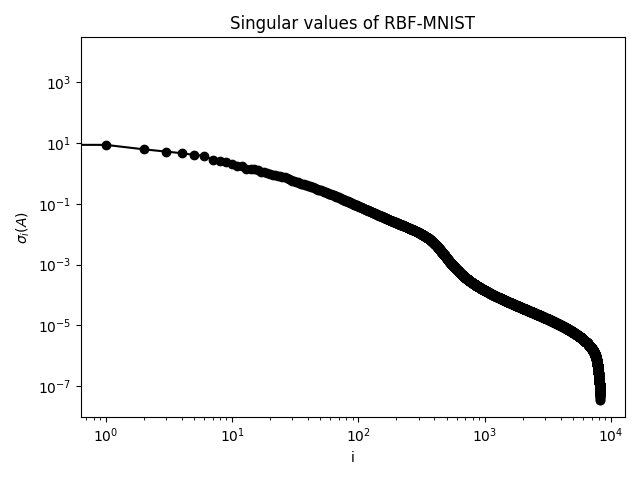
\includegraphics[width=\dimexpr\linewidth-20pt\relax]
        {../plots/singular_values/singular_values_RBF-MNIST.png}
\end{subfigure}\
\begin{subfigure}[t]{\dimexpr0.35\textwidth+20pt\relax}
    \makebox[20pt]{\raisebox{65pt}{\rotatebox[origin=c]{90}{YearMSD, $\sigma=10^4$}}}%
    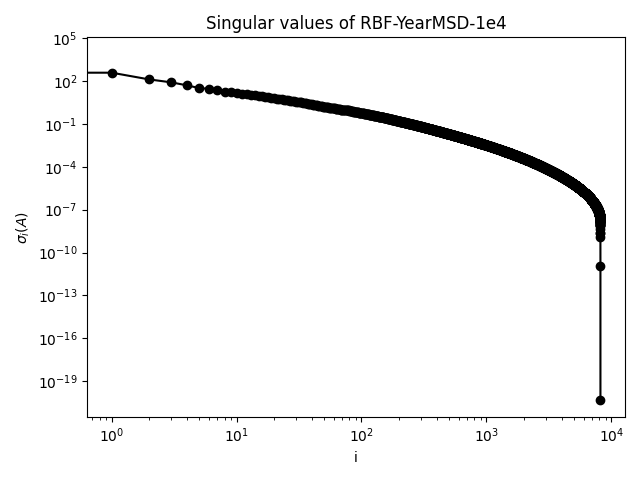
\includegraphics[width=\dimexpr\linewidth-20pt\relax]
        {../plots/singular_values/singular_values_RBF-YearMSD-1e4.png}
\end{subfigure}
\begin{subfigure}[t]{\dimexpr0.35\textwidth+20pt\relax}
    \makebox[20pt]{\raisebox{65pt}{\rotatebox[origin=c]{90}{YearMSD, $\sigma=10^5$}}}%
    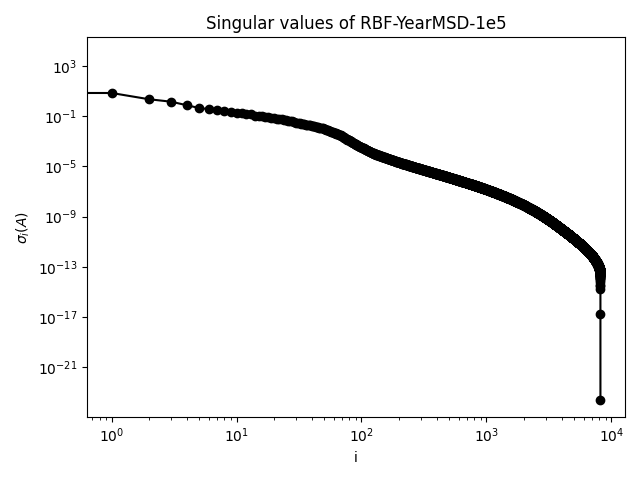
\includegraphics[width=\dimexpr\linewidth-20pt\relax]
        {../plots/singular_values/singular_values_RBF-YearMSD-1e5.png}
\end{subfigure}
\begin{subfigure}[t]{\dimexpr0.35\textwidth+20pt\relax}
    \makebox[20pt]{\raisebox{65pt}{\rotatebox[origin=c]{90}{Polynomial decay}}}%
    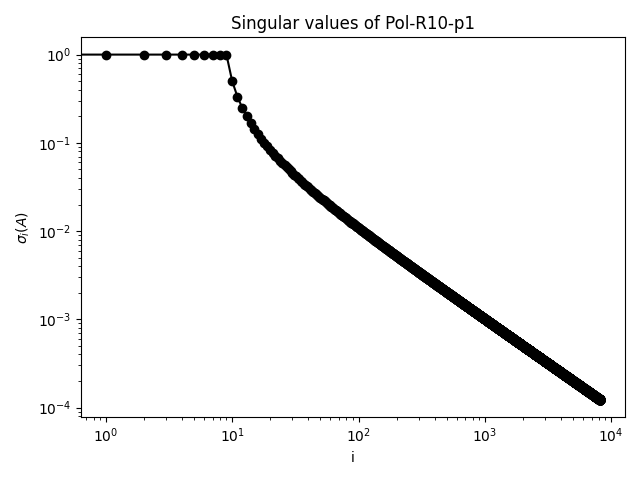
\includegraphics[width=\dimexpr\linewidth-20pt\relax]
        {../plots/singular_values/singular_values_Pol-R10-p1.png}
\end{subfigure}
\begin{subfigure}[t]{\dimexpr0.35\textwidth+20pt\relax}
    \makebox[20pt]{\raisebox{65pt}{\rotatebox[origin=c]{90}{Exponential decay}}}%
    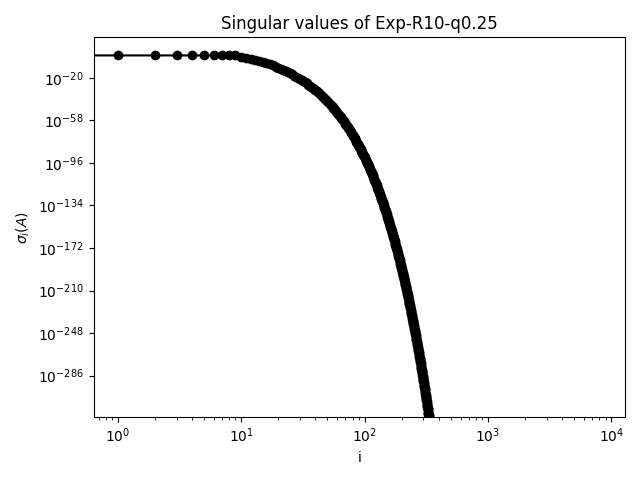
\includegraphics[width=\dimexpr\linewidth-20pt\relax]
        {../plots/singular_values/singular_values_Exp-R10-q0.25.png}
\end{subfigure}
\caption{Singular values of the datasets.}
\label{fig:singularValue}
\end{wrapfigure}

The sketching algorithm works by first computing $C$ and then using $C$ to
compute $B$. Algorithm \ref{algo:sketching} illustrates the procedure. For each
processor owning a block $A_{ij} \in \mathbb{R}^{n/\!\sqrt{P} \times
n/\!\sqrt{P}}$, we start by generating the corresponding block $\Omega_j \in
\mathbb{R}^{n/\!\sqrt{P} \times l}$ of the sketching matrix. Then, we compute
$C_{ij} = A_{ij} \Omega_j$ in parallel and sum-reduce among processors in the
same row $C_i = \sum_{j = 1}^{\sqrt{P}} C_{ij}$. For the computation of $B$, we
need to sketch each $C_i$ from the left by multiplying $\Omega_i$. Note that for
processors owning a diagonal block $A_{ii}$, it holds $\Omega_i = \Omega_j$ and
we do not have to generate $\Omega_i$. Therefore, we choose the processors
owning a diagonal block $A_{ii}$ of $A$ as roots for the reduce operation. Now,
we could simply compute $\Omega_i^T C_i$ on the $\sqrt{P}$ processors owning a
$C_i$ block and then sum-reduce among these to obtain $B$. However, later we
want to execute the TSQR algorithm on all $P$ processors using a row-block
distribution of $C$. Therefore, we chose to scatter $C$ already during sketching
and exploit the additional processing power for the computation of $B$. We
scatter each $C_i$ among processors in the same column because these processors
do all own the same sketching matrix $\Omega_i$. Since we partitioned $C_i \in
\mathbb{R}^{n/\!\sqrt{P} \times l}$ into $C_{ki} \in \mathbb{R}^{n/P \times l}$,
each processor uses only a row-block of $\Omega_i$ for sketching and has to
compute $B_{ki} = \Omega_{ki}^T C_{ki}$. Finally, we sum-reduce $B = \sum_{k,i =
1}^{\sqrt{P}, \sqrt{P}} B_{ki}$ among all processors. Note that the matrix $C$
is row-block distributed and $B$ is owned exclusively by the root processor
after sketching.

Next, the decomposition of $B= LL^T$ is computed sequentially only on the root
processor. The matrix $L$ is then broadcasted to compute $Z = C L^{-T}$ in
parallel. The algebra for 4 processors is:
\begin{align*}
    Z = C L^{-T}
    = \begin{pmatrix}
        C_1 \\
        C_2 \\
        C_3 \\
        C_4
    \end{pmatrix}
    L^{-T}
    = \begin{pmatrix}
        C_1 L^{-T} \\
        C_2 L^{-T} \\
        C_3 L^{-T} \\
        C_4 L^{-T}
    \end{pmatrix}
\end{align*}

Here we utilize that $C_i L^{-T}$ can be found by solving a linear system, thus
never having to find $L^{-1}$. The advantage of the parallelized approach is
that we do not need to gather $C$ together and can compute $Z$ directly
distributed row-block wise which we need anyway for the TSQR algorithm in the
next step.\newline

In the third step, we compute the $QR$ factorization of the tall and skinny
matrix $Z$. We use the (parallel) TSQR algorithm which uses a reduction-like
operation among a binary tree of processors to compute $Q$ and $R$ in parallel
(the binary tree is the reason why we need $P$ being a power of 2). It is
communication optimal and as stable as Householder $QR$. For details, we refer
to \cite{demmel2008}. At the end, the $Q$ factor is returned distributed
row-block wise while $R$ is owned by the root processor.\newline

In the final step, we copute the rank-k truncated SVD $U_k \Sigma_k V_k^T$ of
$R$ and $\Sigma_k^2$ sequentially on the root processor. Then, we broadcast
$U_k$ to compute $\hat{U}_k = Q U_k$ in parallel ($Q$ is still row-block
distributed) and gather $\hat{U}_k$ together. We return $\Sigma_k^2$ as well as
$\hat{U}_k$ on the root processor.

\section{Datasets}\label{sec:datasets}

In the following sections, we will investigate the performance of the Nyström
algorithm on 5 different datasets. The positive semi-definite matrices, $A$,
will be made from both real and synthetic data, as described below. For all
datasets we chose to subsample the datapoints for the real data, or simply
choose the dimension for the synthetic data such that we had $n=8.192$, leading
to a positive semi-definite matrix $A\in\mathbb{R}^{n\times n}$. Note that the
side lengths of $A$, i.e. ($n$), should be divisible by $P$, i.e. a power of $4$
(see Section \ref{sec:parallel_nystrom}). Thus setting $n=2^{13}$ satisfies both
this requirement for $P=4$ and the fact that the SRHT matrices require $n$ as a
power of $2$. You can always satisfy the requirements for $n$ by zero-padding
the input data. \newline

In all experiments, all datasets were run with the different sketching matrices
($\Omega$), sketching dimensions ($l$), and approximation ranks ($k$). We had a
total of 19 different $(l,k)$ pairs with $l\in\{400, 600, 1000, 2000\}$ and
$k\in\{100, 200, 350, 500, 700, 900\}$. Note that this choice of parameters is
specific to us using $P=4$ processors with TSQR. This enables us to use the
\textit{tall and skinny} QR algorithm computing the thin $QR$ factorization of
$Z\in\mathbb{R}^{n\times l}$ for all our parameters since $n\geq 4\cdot
l$.\newline

For the matrices created from real data, we used the MNIST (normalized to have
values in the range $[0,1]$) and YearPredictionMSD datasets \cite{726791,
Bertin-Mahieux2011}. We then used a subset of $n$ datapoints and used the radial
basis function (RBF), $A_{ij}=e^{-||x_i-x_j||_2^2}/{\sigma^2}$ to create a
symmetric and positive semi-definite matrix. For MNIST, we chose a value of
$\sigma=100$, and for YearPredictionMSD we chose $\sigma=10^4$ and $\sigma=10^5$
for a total of 3 datasets, matching the approach in \cite{balabanov2022}. These
datasets will in the following be referred to as \texttt{MNIST},
\texttt{YearMSD-1e4}, and \texttt{YearMSD-1e5}, respectively. \newline
For the synthetic datasets, we choose diagonal matrices containing positive
elements with different rates of decay for the singular values. Since $A$ is a
diagonal matrix, we can easily select the singular values, and thus also choose
an effective rank, $R$, of the matrices. We used both a \textit{Polynomial
decay} and an \textit{Exponential decay} of the singular values. The matrix with
\textit{Polynomial decay} has the form\\
\begin{equation*}
A=\text{diag}(\underbrace{1,...,1}_R,2^{-p}, 3^{-p}, ..., (n-R+1)^{-p})\in\mathbb{R}^{n\times n}.
\end{equation*}
The parameter $p>0$ is a hyperparameter used to control the decay of the
polynomially decaying singular values. The matrix with \textit{Exponential
decay} has the form
\begin{equation*}
A=\text{diag}(\underbrace{1,...,1}_R,10^{-q}, 10^{-2q}, ..., 10^{-(n-R)q})\in\mathbb{R}^{n\times n}
\end{equation*}
The parameter $q>0$ again controls the rate of decay, now of the exponentially
decaying singular values. To match the datasets in \cite{tropp2017fixedrank}, we
set $R=10$, $p=1$, and $q=0.25$ for all experiments, also matching the real
datasets in size by setting $n=8.192$, leading to 2 synthetic datasets, referred
to as \texttt{Polynomial} and \texttt{Exponential}.

To investigate the datasets, Figure \ref{fig:singularValue} displays the decay
of the singular values for the $A$ matrices. We computed the singular values via
the SVD for the real datasets, and via the diagonal elements for the diagonal
matrices. Looking firstly at the synthetic datasets, we see that a polynomial
decay in singular values leads to a straight line, maybe even a bit of curvature
upwards, in a log-log plot with the smallest singular values at $10^{-4}$. On
the other hand, the exponential dataset has a downward curvature on the singular
values in the log-log plot with the smallest singular values being less than
machine precision. With these two (synthetic) decays in mind, we can take a look
at the datasets created by the RBF kernel. For all of them, we see a curvature
downward on the singular values indicating a decay faster than a polynomial
decay. We see very similar decay and magnitude between the \texttt{MNIST} and
\texttt{YearMSD-1e4} (ignoring the very last singular value), but find that for
\texttt{YearMSD-1e5} (simply adjusting $\sigma$), we have significantly smaller
singular values and even have similar behavior to \texttt{Exponential} for the
singular values above $i=1000$. If we were to find the best rank $k$
approximation to these datasets and get a $2$-norm error below $10^{-5}$, we
would expect to use an approximation rank of a few thousand for
\texttt{YearMSD-1e4} and \texttt{MNIST}, a rank of a few hundred for
\texttt{YearMSD-1e5}, a rank of less than 100 for \texttt{Exponential}, whereas
no approximation could be found for \texttt{Polynomial}.

\section{Numerical Stability} \label{sec:num_stability}
%  An investigation of the numerical stability of randomized Nystr¨om. For the
%  data sets described in section 2.1, you should provide graphs that display
%  the error of the low rank approximation in terms of nuclear norm (norm(A,
%  'nuc')). The error to be studied experimentally is kA−[[ANyst]]kk∗/kAk∗. The
%  discussion should compare as well the accuracy obtained for the two different
%  sketching matrices by taking into consideration the sketching dimension. This
%  investigation should be done on the data sets provided in 2.1. Additional
%  data could be provided but is not required.

For the numerical analysis and the performance evaluation, we executed all
experiments on a single machine with an Intel Core i5 6500 ($4 \times 3.6$ GHz,
$6$MB L3 cache) processor and 16 GB of DDR4-RAM powered by Fedora 38 (64-Bit,
Linux Kernel $6.5.6$). Furthermore, the algorithms have been implemented in
Python $3.11.5$ using NumPy $1.26.0$. The parallelization has been done via the
Python implementation \textit{mpi4py} $3.1.4$ of the well-known Message Passing
Interface (MPI) (OpenMPI 4.1.4). The machine precision is $2.220446049250313
\cdot 10^{-16}$ for the type \textit{float} (or \textit{single precision}) on
our system. Moreover, we limit the threads available to the BLAS (Basic Linear
Algebra Subprograms) library used by NumPy to 1.\newline

The numerical performance is tested on the datasets described in Section
\ref{sec:datasets}. The performance is measured using the relative error with
the nuclear norm,
\begin{equation}
    \textit{Relative error: } \frac{||A-\llbracket A_{nyst}\rrbracket_k||_*}{||A||_*}.
\end{equation}
Since the nuclear norm is the sum of the singular values,
$||A||_*=\sigma_1(A)+...+\sigma_n(A)$, this value describes the ratio of the sum
of the singular values from the approximation error of $\llbracket
A_{nyst}\rrbracket_k$, compared to the original matrix $A$. If this value is
low, we have a good low-rank approximation of $A$. \newline

We used the parallel randomized Nyström with Cholesky for all datasets except
for \texttt{Exponential}. For this dataset, Cholesky failed since $B$ was
classified as a singular matrix. It also makes sense that \texttt{Exponential}
would run into problems with singular matrices when looking at the decay of the
singular values in Figure \ref{fig:singularValue}, as its singular values are
significantly lower than for the other datasets. For this dataset, we instead
used the SVD approach. Because of the runtime differences, as seen in Section
\ref{sec:performance}, we chose to use the SVD approach only for this
dataset.\newline

The relative error for all datasets and both sketching matrices can be seen in
Figure \ref{fig:RelError}. For all the tests except for \texttt{Exponential}, we
could see a monotonic reduction in relative error using a larger size of $l$ or
$k$, if the other value was kept fixed. However, when keeping $l$ fixed, even
though the relative error was reduced when increasing $k$, we found a reduction
in the improvement for each step. That is, we get diminishing returns on the
improvement in the relative error when increasing the approximation rank, $k$.
The exception to this was \texttt{Exponential}, where the effects of changing
the approximation rank or the sketching dimension were inconclusive. However,
for all tests run with \texttt{Exponential}, the relative error was close to or
below $10^{-14}$, which is nearing machine precision, and significantly lower
than all other considered datasets. \newline

Comparing across the different datasets, we see a big difference in the
magnitude of the relative errors. \texttt{Polynomial} has a much larger relative
error, compared to all other datasets, and \texttt{YearMSD-1e5} is significantly
better than all other datasets (except \texttt{Exponential} mentioned before),
across all combinations of different hyperparameters. This also shows that for
the YearPredictionMSD dataset, the value for $\sigma$ has a much larger impact
on the relative error than the values for the sketching dimension or the
approximation rank. It seems that datasets created with a smaller standard
deviation in the radial basis function, are easier to approximate using the
randomized Nyström approximation. However, in general, for the correct value of
$\sigma$, the randomized Nyström algorithm works well in combination with kernel
methods using the RBF kernel. \newline

Comparing with the decay of the singular values in Figure
\ref{fig:singularValue}, we find a close relationship between the decay of the
singular values and the numerical relative error. The datasets with the fastest
decay of singular values have the lowest relative error. Since we are working
with a fixed-rank approximation, this is to be expected, as a slow decay of
singular values makes the matrix harder to approximate with a low-rank
approximation. Assuming best-rank approximation, $\llbracket A\rrbracket_k$, we
have that for a dataset like \texttt{Polynomial}, with a large tail of singular
values, it should have a worse performance than for \texttt{Exponential}, where
a low-rank approximation results in a small error on the singular
values.\newline

Another interesting finding across datasets is that when fixing a low
approximation error, the difference in relative error when varying the sketching
dimension, depended heavily on the initial performance. That is, if we found a
low relative error for a low approximation rank, increasing the sketch dimension
made little to no difference, but when the initial performance was poor, as with
\texttt{Polynomial}, we did see some difference. So if one were to select
between increasing the sketch dimension or the approximation rank to get the
most improvement in the relative error, the results were not conclusive.
However, as a general trend, for a low approximation rank, we found the most
improvement by increasing the approximation rank, and for medium to high
approximation ranks we found more significant improvements by increasing the
sketch dimension. This also explains why \texttt{YearMSD-1e5} has a better
performance than the other two RBF datasets, as it has a faster decay on the
singular values with the higher value of $\sigma$.\newline

Comparing across different sketching matrices, we find next to identical
results. That is, in our testing, we did not find any significant numerical
differences between the two different sketching matrices. The only visible
difference across sketching matrices was for the exponential decay dataset, but
the numerical difference is small, and the error for both is close to machine
precision.

% Relative error plots - describe what we see/have found

\begin{figure}
\centering
\hfill\begin{subfigure}[t]{\dimexpr0.4\textwidth+20pt\relax}
    \makebox[20pt]{\raisebox{65pt}{\rotatebox[origin=c]{90}{MNIST}}}%
    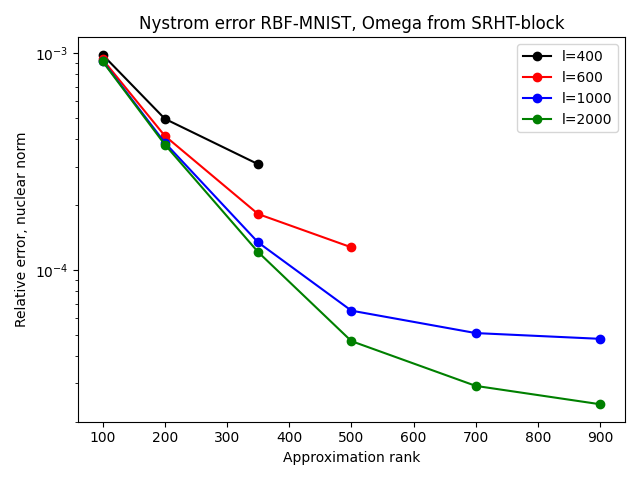
\includegraphics[width=\dimexpr\linewidth-20pt\relax]
        {../plots/relerror/relerror_RBF-MNIST_SRHT-block.png}
    \makebox[20pt]{\raisebox{65pt}{\rotatebox[origin=c]{90}{YearMSD, $\sigma=10^4$}}}%
    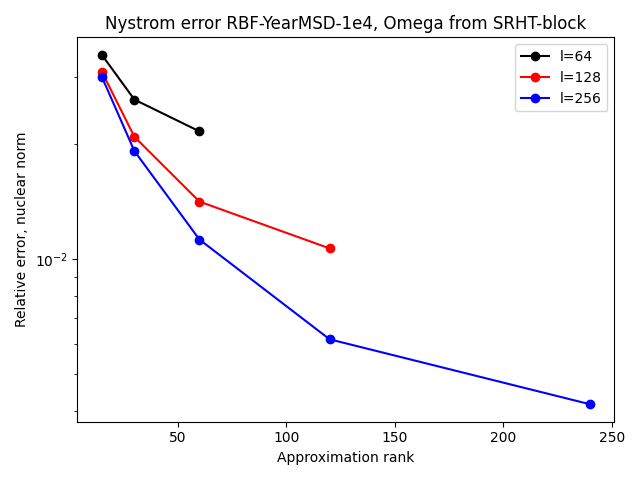
\includegraphics[width=\dimexpr\linewidth-20pt\relax]
        {../plots/relerror/relerror_RBF-YearMSD-1e4_SRHT-block.png}
    \makebox[20pt]{\raisebox{65pt}{\rotatebox[origin=c]{90}{YearMSD, $\sigma=10^5$}}}%
    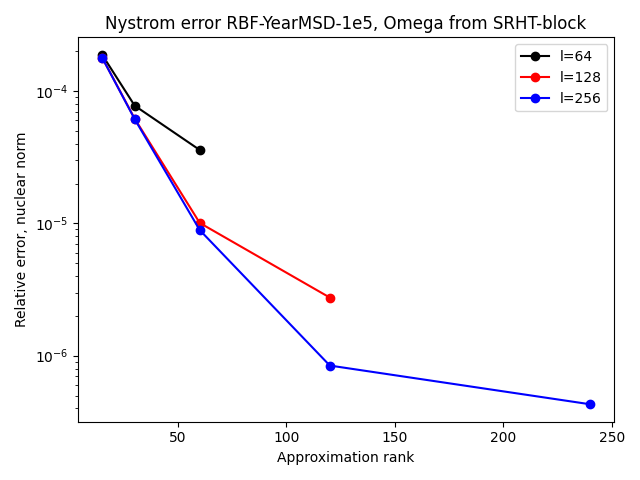
\includegraphics[width=\dimexpr\linewidth-20pt\relax]
        {../plots/relerror/relerror_RBF-YearMSD-1e5_SRHT-block.png}
    \makebox[20pt]{\raisebox{65pt}{\rotatebox[origin=c]{90}{Polynomial decay}}}%
    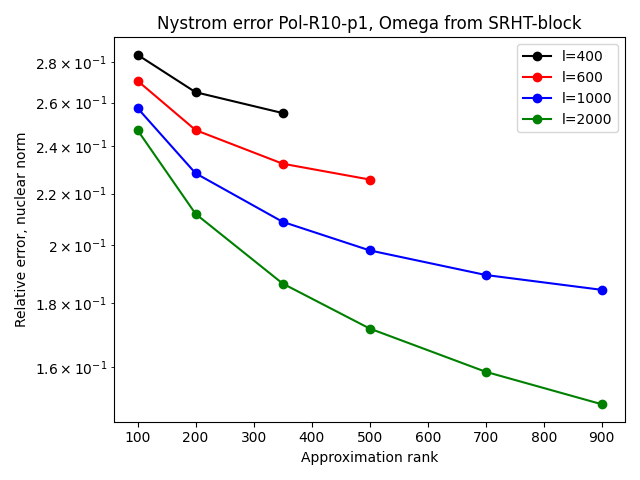
\includegraphics[width=\dimexpr\linewidth-20pt\relax]
        {../plots/relerror/relerror_Pol-R10-p1_SRHT-block.png}
    \makebox[20pt]{\raisebox{65pt}{\rotatebox[origin=c]{90}{Exponential decay}}}%
    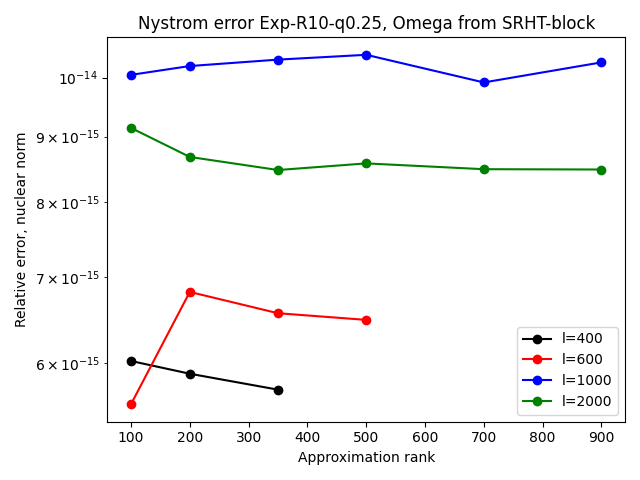
\includegraphics[width=\dimexpr\linewidth-20pt\relax]
        {../plots/relerror/relerror_Exp-R10-q0.25_SRHT-block.png}
    \caption{$\Omega$ created using BSRHT}
\end{subfigure}\hfill
\begin{subfigure}[t]{0.4\textwidth}
    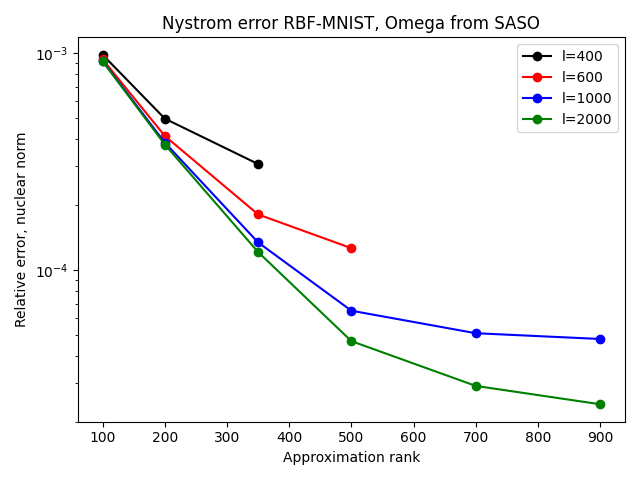
\includegraphics[width=\textwidth]
        {../plots/relerror/relerror_RBF-MNIST_SASO.png}
    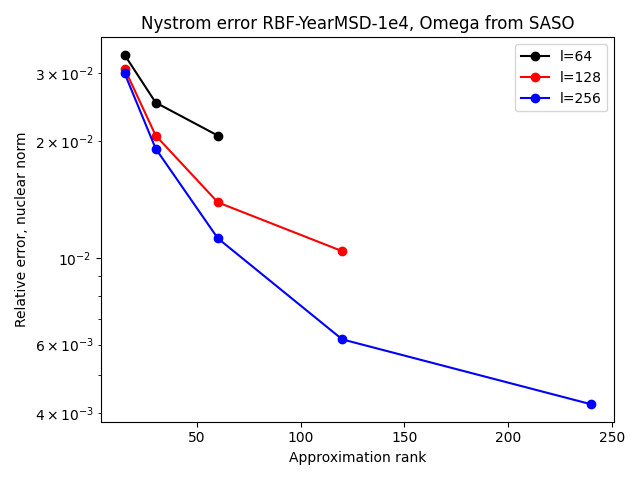
\includegraphics[width=\textwidth]
        {../plots/relerror/relerror_RBF-YearMSD-1e4_SASO.png}
    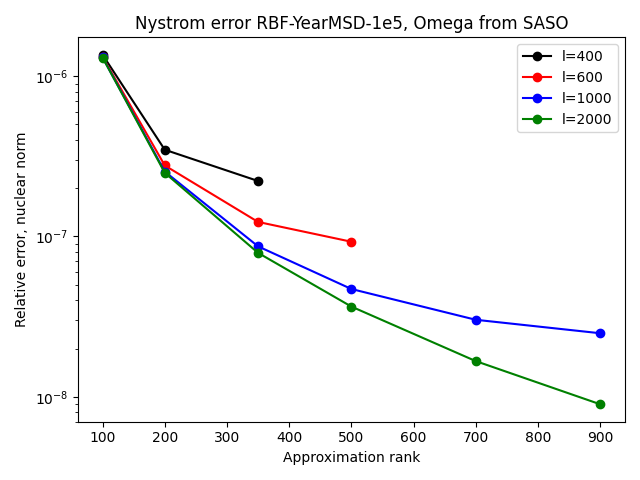
\includegraphics[width=\textwidth]
        {../plots/relerror/relerror_RBF-YearMSD-1e5_SASO.png}
    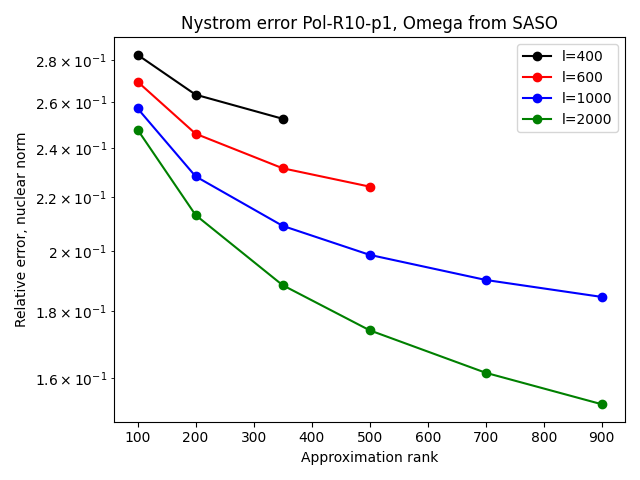
\includegraphics[width=\textwidth]
        {../plots/relerror/relerror_Pol-R10-p1_SASO.png}
    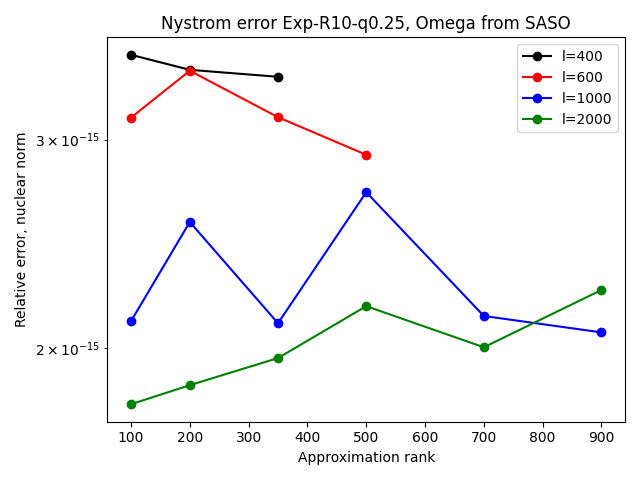
\includegraphics[width=\textwidth]
        {../plots/relerror/relerror_Exp-R10-q0.25_SASO.png}
    \caption{$\Omega$ created using SASO}
\end{subfigure}\hfill
\caption{Relative error of the Nyström algorithm.}
\label{fig:RelError}
\end{figure}

\section{Runtime} \label{sec:performance}

We evaluated the runtime of the randomized Nyström algorithm on the same
parameters as in Section \ref{sec:num_stability}. The runtime was measured as
the time to do the steps described in Sections \ref{sec:rand_nystrom_alg} and
\ref{sec:parallel_nystrom}, and thus does not include the time to generate the
positive semi-definite matrix $A$ from the data, as is required when using
kernel methods. To quantify the variation in runtimes, all tests were run 5
times to show the mean and the standard deviation of the runtimes at the
different parameters.\newline


\subsection{Parallel runtime}
The parallel runtime, with the sketching matrices created using BSRHT and SASO,
are shown in Figure \ref{fig:Runtime}. We find that \texttt{Exponential} is
significantly slower to run than the other datasets. This difference comes down
to the difference between the algorithms used, as the SVD approach has a higher
computational cost, as described in Section \ref{sec:rand_nystrom_alg}. Besides
the difference found between the two algorithms, we found little variation in
the runtime across datasets. \newline

When selecting between the sketching dimension and the approximation rank, we
see a large difference in runtimes. When increasing the sketching dimension, and
thus working with larger sketched matrices $B$ and $C$, it takes significantly
longer to run the approximation. We consistently saw an increase of runtime of
more than a factor 3 when doubling the sketching dimension from $1000$ to
$2000$. We also found that the increase in runtime when increasing the sketch
dimension was larger than any of our increases in the approximation rank. This
makes sense when looking back at Section \ref{sec:parallel_nystrom}, where an
increase in sketching dimension is directly related to the size of the matrices,
$C_i\in\mathbb{R}^{n/\!\sqrt{P}\times l}$ and $B_{ij}\in\mathbb{R}^{l\times l}$,
and thus the size of matrices that we find the Cholesky/SVD decomposition of in
the parallel randomized Nyström algorithm. On the other hand, the difference in
runtime across the approximation rank only affects the final step described in
Section \ref{sec:parallel_nystrom}, where the rank-k truncated SVD is found, and
the $\llbracket A_{Nyst}\rrbracket_k$ is calculated. Therefore, we conclude that
the sketching dimension has the largest effect on the runtime of the randomized
Nyström algorithm.

% No Q vs Q version. Describe our choice
% Runtime plots - describe what we see/have found

\begin{figure}
\centering
\hfill\begin{subfigure}[t]{\dimexpr0.4\textwidth+20pt\relax}
    \makebox[20pt]{\raisebox{65pt}{\rotatebox[origin=c]{90}{MNIST}}}%
    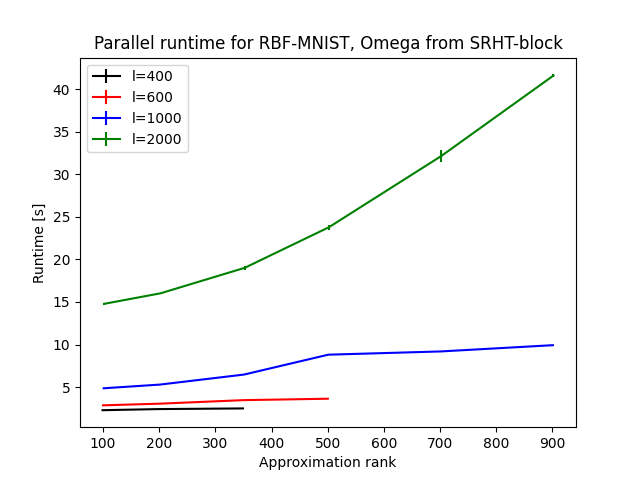
\includegraphics[width=\dimexpr\linewidth-20pt\relax]
        {../plots/runtime_new/runtime_par_RBF-MNIST_SRHT-block.png}
    \makebox[20pt]{\raisebox{65pt}{\rotatebox[origin=c]{90}{YearMSD, $\sigma=10^4$}}}%
    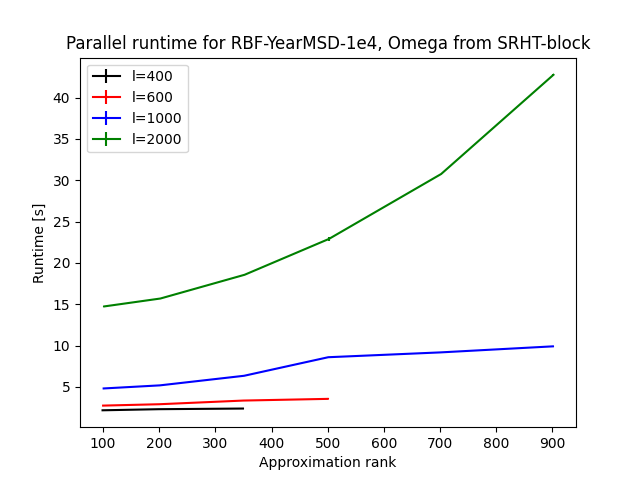
\includegraphics[width=\dimexpr\linewidth-20pt\relax]
        {../plots/runtime_new/runtime_par_RBF-YearMSD-1e4_SRHT-block.png}
    \makebox[20pt]{\raisebox{65pt}{\rotatebox[origin=c]{90}{YearMSD, $\sigma=10^5$}}}%
    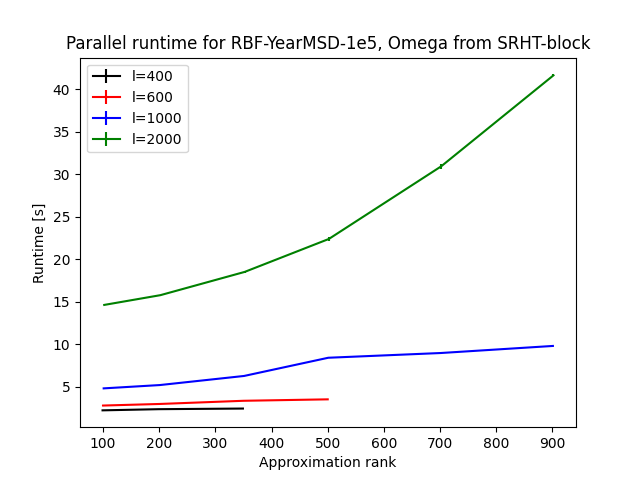
\includegraphics[width=\dimexpr\linewidth-20pt\relax]
        {../plots/runtime_new/runtime_par_RBF-YearMSD-1e5_SRHT-block.png}
    \makebox[20pt]{\raisebox{65pt}{\rotatebox[origin=c]{90}{Polynomial decay}}}%
    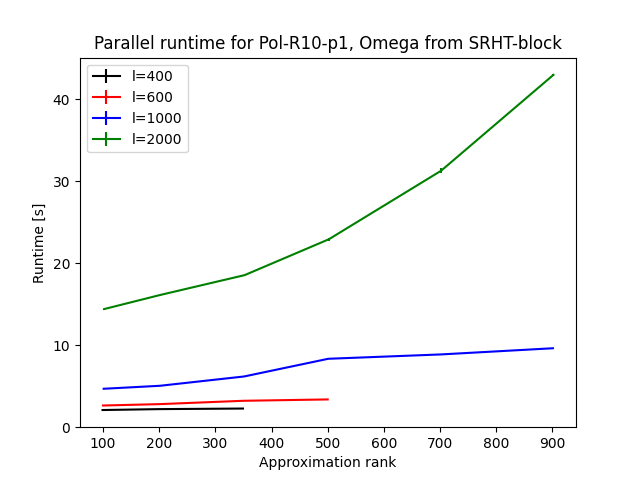
\includegraphics[width=\dimexpr\linewidth-20pt\relax]
        {../plots/runtime_new/runtime_par_Pol-R10-p1_SRHT-block.png}
    \makebox[20pt]{\raisebox{65pt}{\rotatebox[origin=c]{90}{Exponential decay}}}%
    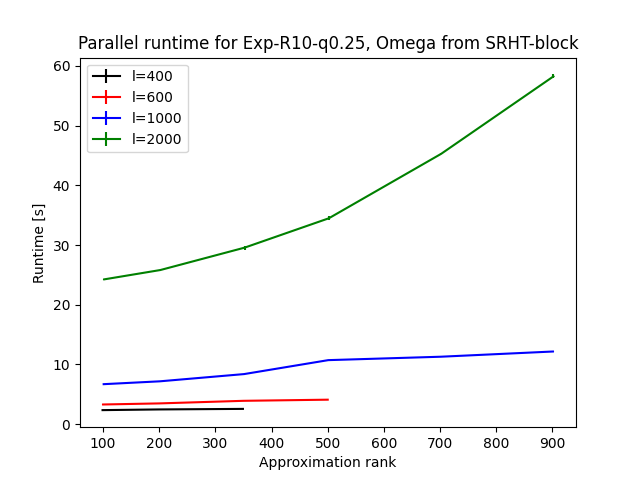
\includegraphics[width=\dimexpr\linewidth-20pt\relax]
        {../plots/runtime_new/runtime_par_Exp-R10-q0.25_SRHT-block.png}
    \caption{$\Omega$ created using BSRHT}
\end{subfigure}\hfill
\begin{subfigure}[t]{0.4\textwidth}
    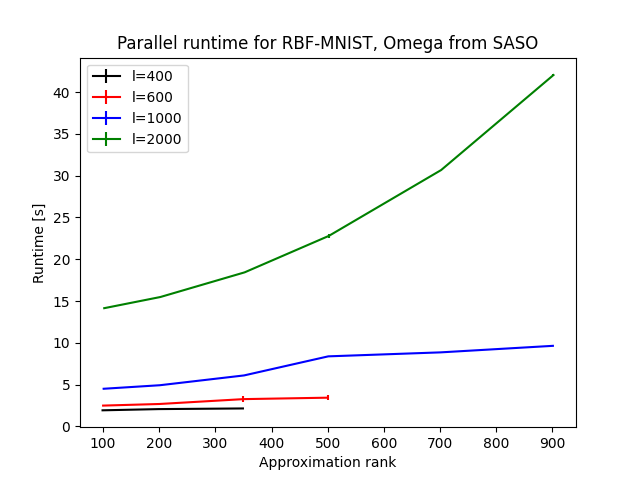
\includegraphics[width=\textwidth]
        {../plots/runtime_new/runtime_par_RBF-MNIST_SASO.png}
    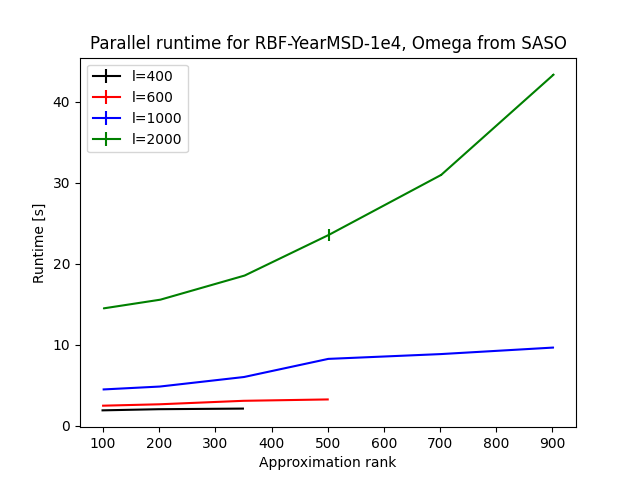
\includegraphics[width=\textwidth]
        {../plots/runtime_new/runtime_par_RBF-YearMSD-1e4_SASO.png}
    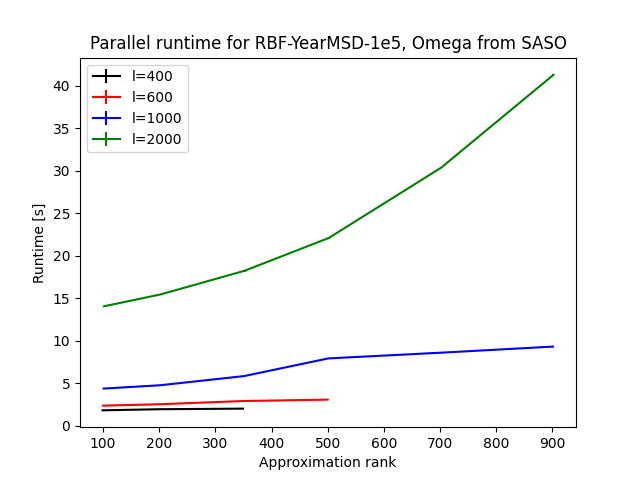
\includegraphics[width=\textwidth]
        {../plots/runtime_new/runtime_par_RBF-YearMSD-1e5_SASO.png}
    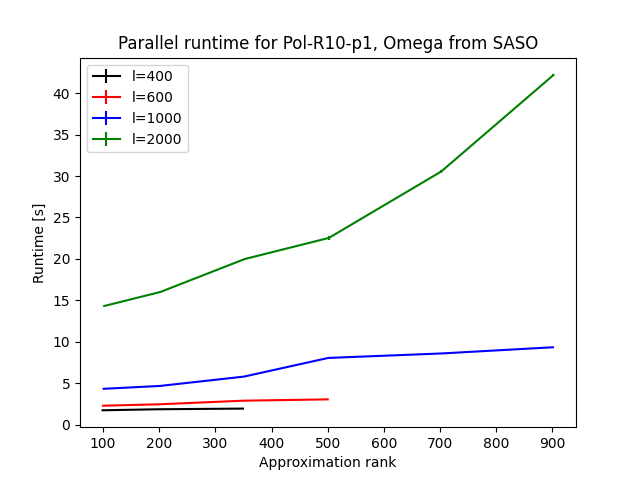
\includegraphics[width=\textwidth]
        {../plots/runtime_new/runtime_par_Pol-R10-p1_SASO.png}
    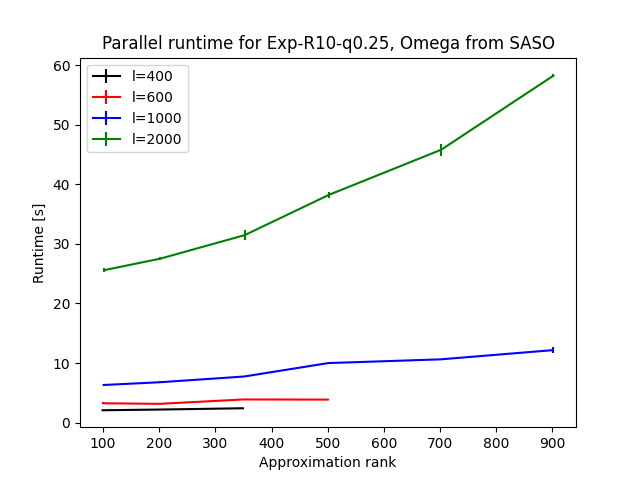
\includegraphics[width=\textwidth]
        {../plots/runtime_new/runtime_par_Exp-R10-q0.25_SASO.png}
    \caption{$\Omega$ created using SASO}
\end{subfigure}\hfill
\caption{Runtime of the parallel Nyström algorithm.}
\label{fig:Runtime}
\end{figure}

\subsection{Sequential runtime}

The sequential runtime, with the sketching matrices created using SRHT and SASO,
are shown in Figure \ref{fig:SequentialRuntime}. We find very similar internal
comparisons between the different datasets. Since \texttt{Exponential} is run
using the SVD approach, this has a much higher runtime than the other datasets.
As with the parallel runtimes, we also see that increasing the approximation
rank or the sketching dimension leads to a higher runtime, with the sketching
dimension having the largest influence.

Comparing against the parallel runtime, we find that going from the parallel
algorithm (with $4$ processors) to the sequential algorithm, the runtime
increases by 30-50\%. Thus switching to the parallel algorithm gives a
significant improvement, especially when the runtime is upwards of $60+$ seconds
for some parameter settings with the sequential algorithm. However, as we have
increased the number of processors by a factor of $4$, our parallelization has
some overhead. Note that we measured the runtime of the parallel algorithm
including scattering the matrix $A$ and gathering $[\![A]\!]_k$ back together
across processors. Ignoring this data distribution would further reduce the
runtime.

% Discuss if you observe any advantage in using a faster sketching operator with
% respect to the sketch dimension l that you might need in order to obtain an
% accurate low rank approximation.
Comparing the two different sketching matrices, we find little to no difference
in runtime between the SRHT and SASO sketching operators. That is, getting a
low-rank approximation, $\llbracket A_{nyst}\rrbracket_k$, is not significantly
affected by the choice between SRHT and SASO. However, we did see a slightly
shorter runtime for SASO than for SRHT for some of the larger runtimes, for
instance for the \texttt{YearMSD-1e5} with the highest approximation rank and
sketching dimension. Since we have seen in the previous section that both
sketching operators produce similar results w.r.t. accuracy, the SASO is the
preferable choice for our test matrices when looking only at the running time.

\begin{figure}
\centering
\hfill\begin{subfigure}[t]{\dimexpr0.4\textwidth+20pt\relax}
    \makebox[20pt]{\raisebox{65pt}{\rotatebox[origin=c]{90}{MNIST}}}%
    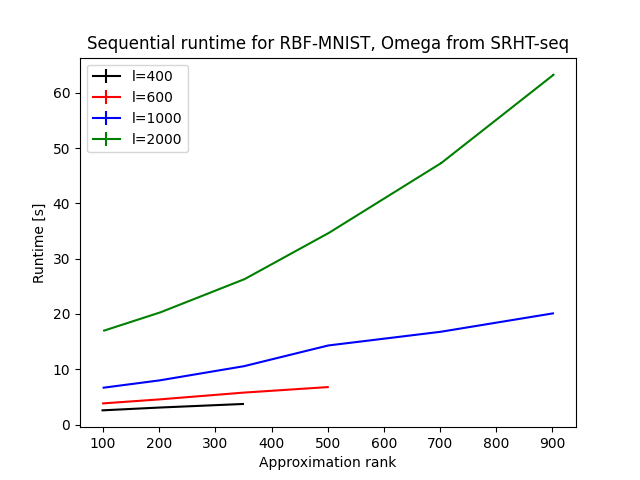
\includegraphics[width=\dimexpr\linewidth-20pt\relax]
        {../plots/runtime_new/runtime_RBF-MNIST_SRHT-seq.png}
    \makebox[20pt]{\raisebox{65pt}{\rotatebox[origin=c]{90}{YearMSD, $\sigma=10^4$}}}%
    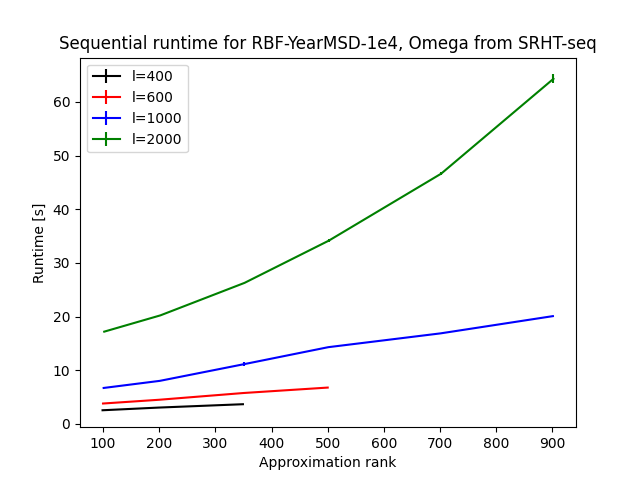
\includegraphics[width=\dimexpr\linewidth-20pt\relax]
        {../plots/runtime_new/runtime_RBF-YearMSD-1e4_SRHT-seq.png}
    \makebox[20pt]{\raisebox{65pt}{\rotatebox[origin=c]{90}{YearMSD, $\sigma=10^5$}}}%
    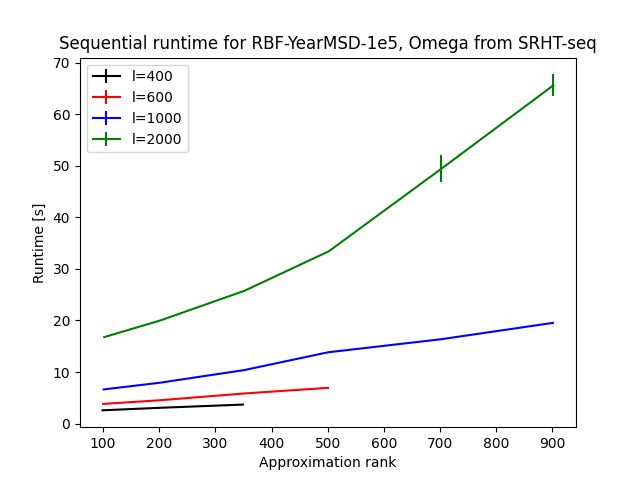
\includegraphics[width=\dimexpr\linewidth-20pt\relax]
        {../plots/runtime_new/runtime_RBF-YearMSD-1e5_SRHT-seq.png}
    \makebox[20pt]{\raisebox{65pt}{\rotatebox[origin=c]{90}{Polynomial decay}}}%
    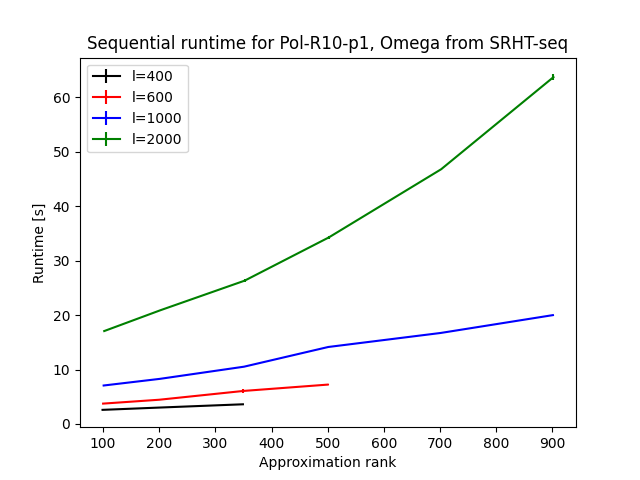
\includegraphics[width=\dimexpr\linewidth-20pt\relax]
        {../plots/runtime_new/runtime_Pol-R10-p1_SRHT-seq.png}
    \makebox[20pt]{\raisebox{65pt}{\rotatebox[origin=c]{90}{Exponential decay}}}%
    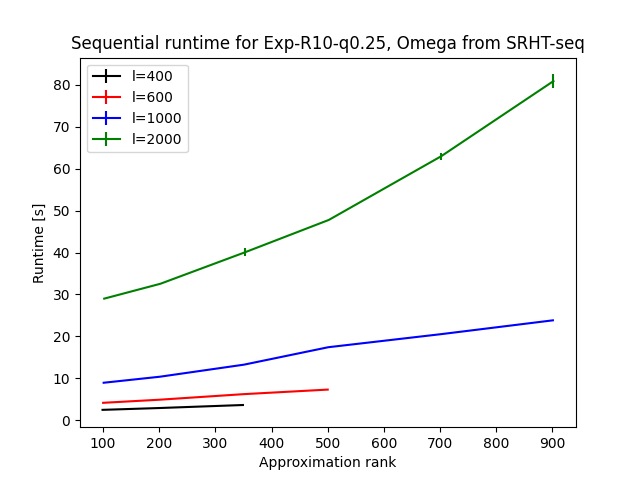
\includegraphics[width=\dimexpr\linewidth-20pt\relax]
        {../plots/runtime_new/runtime_Exp-R10-q0.25_SRHT-seq.png}
    \caption{$\Omega$ created using SRHT}
\end{subfigure}\hfill
\begin{subfigure}[t]{0.4\textwidth}
    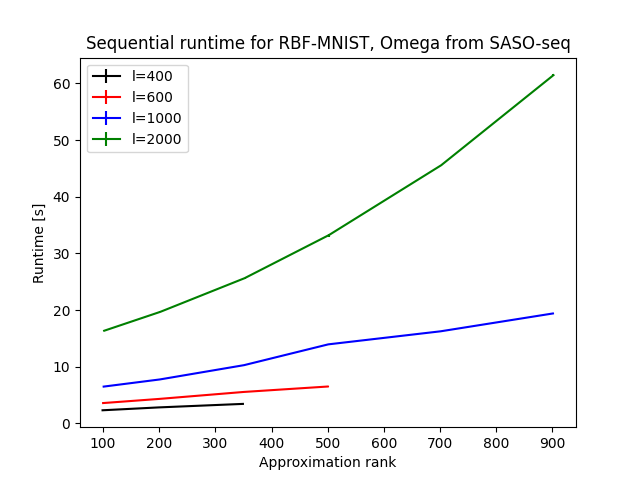
\includegraphics[width=\textwidth]
        {../plots/runtime_new/runtime_RBF-MNIST_SASO-seq.png}
    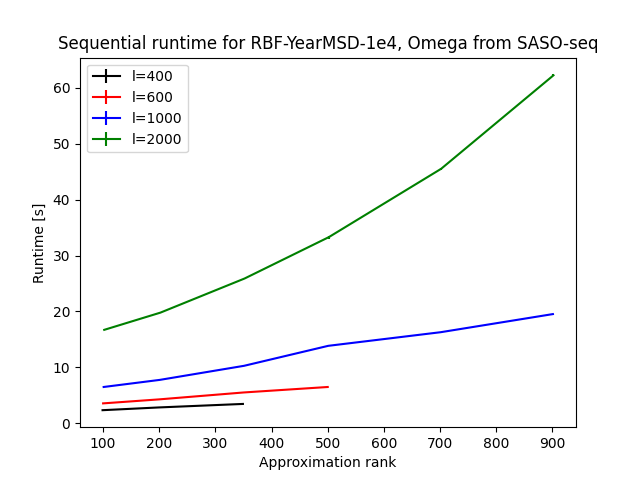
\includegraphics[width=\textwidth]
        {../plots/runtime_new/runtime_RBF-YearMSD-1e4_SASO-seq.png}
    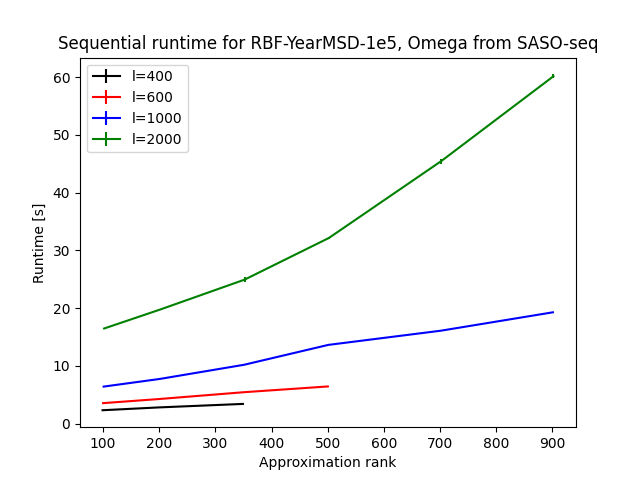
\includegraphics[width=\textwidth]
        {../plots/runtime_new/runtime_RBF-YearMSD-1e5_SASO-seq.png}
    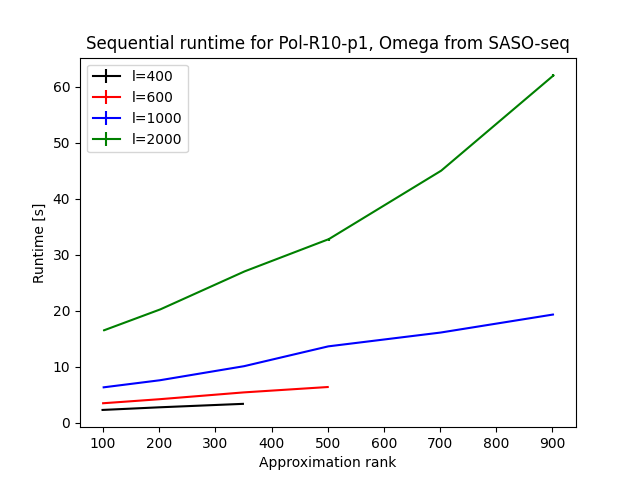
\includegraphics[width=\textwidth]
        {../plots/runtime_new/runtime_Pol-R10-p1_SASO-seq.png}
    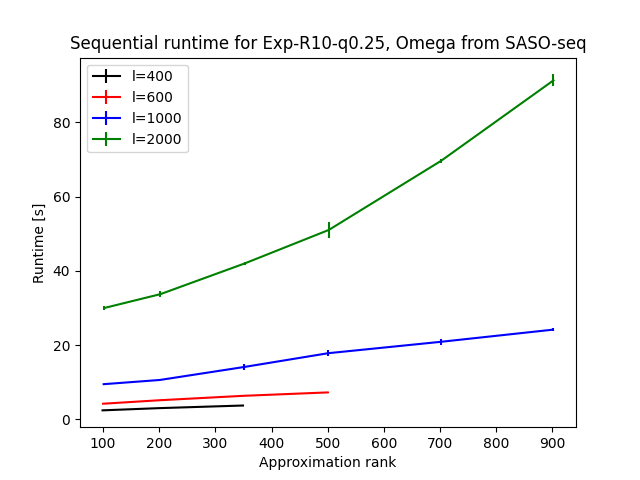
\includegraphics[width=\textwidth]
        {../plots/runtime_new/runtime_Exp-R10-q0.25_SASO-seq.png}
    \caption{$\Omega$ created using SASO}
\end{subfigure}\hfill
\caption{Runtime of the sequential version of the randomized Nyström algorithm.}
\label{fig:SequentialRuntime}
\end{figure}

\begin{figure}
\centering
\hfill\begin{subfigure}[t]{\dimexpr0.4\textwidth+20pt\relax}
    \makebox[20pt]{\raisebox{65pt}{\rotatebox[origin=c]{90}{MNIST}}}%
    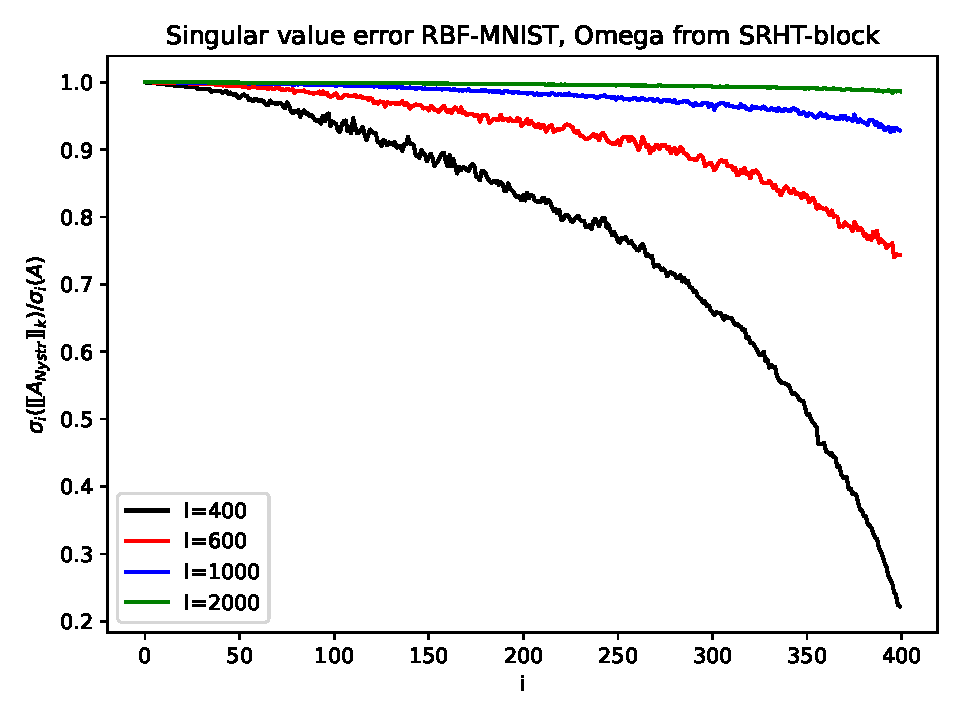
\includegraphics[width=\dimexpr\linewidth-20pt\relax]
        {../plots/singular_values/singular_values_RBF-MNIST_SRHT-block.pdf}
    \makebox[20pt]{\raisebox{65pt}{\rotatebox[origin=c]{90}{YearMSD, $\sigma=10^4$}}}%
    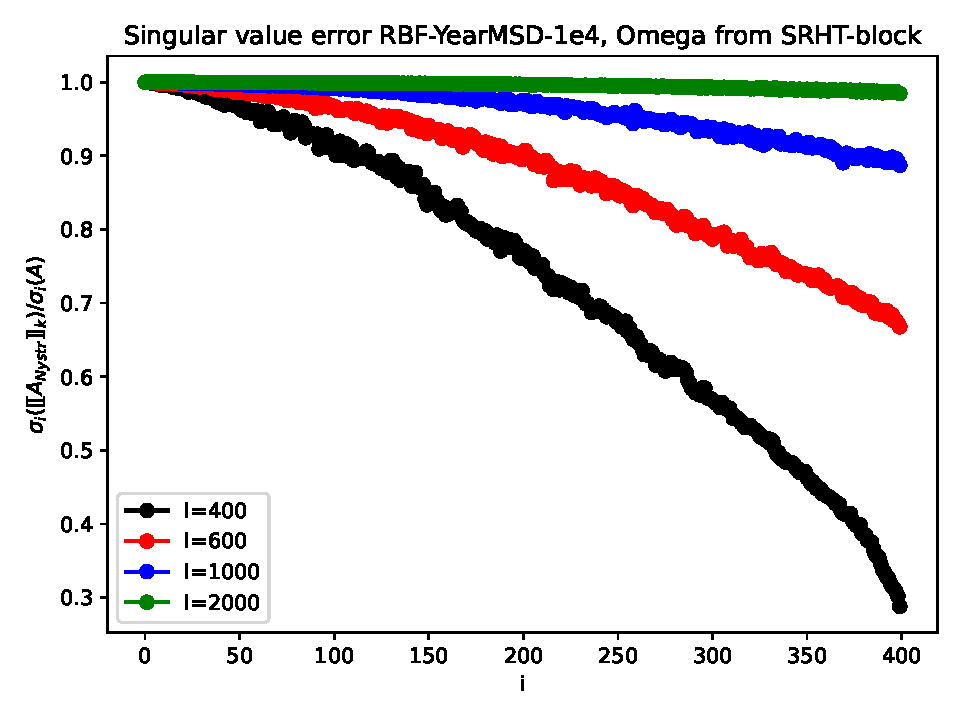
\includegraphics[width=\dimexpr\linewidth-20pt\relax]
        {../plots/singular_values/singular_values_RBF-YearMSD-1e4_SRHT-block.pdf}
    \makebox[20pt]{\raisebox{65pt}{\rotatebox[origin=c]{90}{YearMSD, $\sigma=10^5$}}}%
    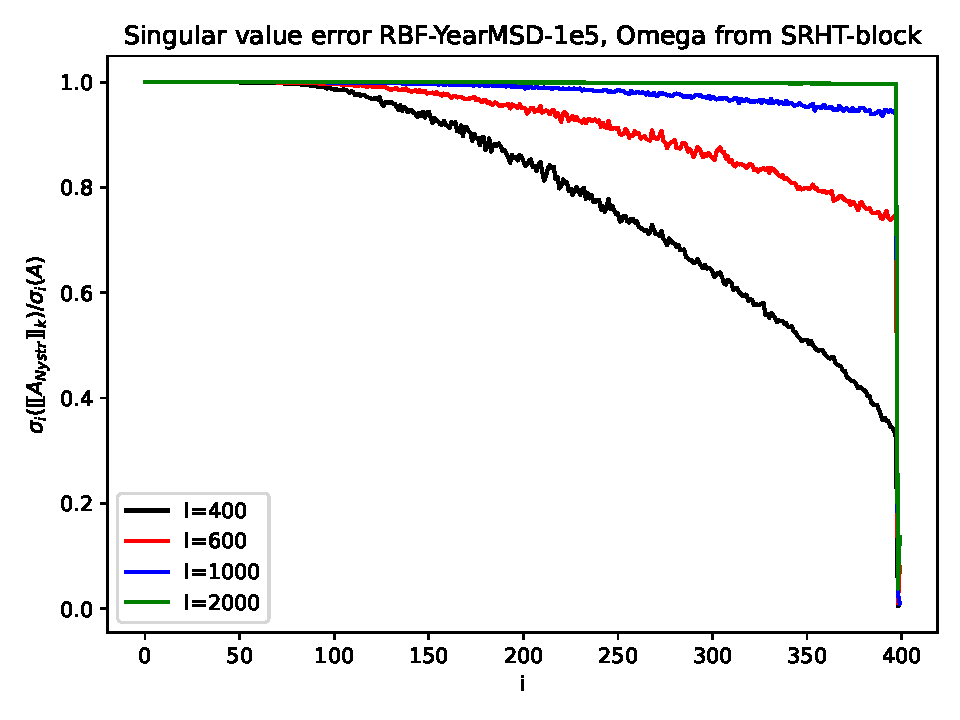
\includegraphics[width=\dimexpr\linewidth-20pt\relax]
        {../plots/singular_values/singular_values_RBF-YearMSD-1e5_SRHT-block.pdf}
    \makebox[20pt]{\raisebox{65pt}{\rotatebox[origin=c]{90}{Polynomial decay}}}%
    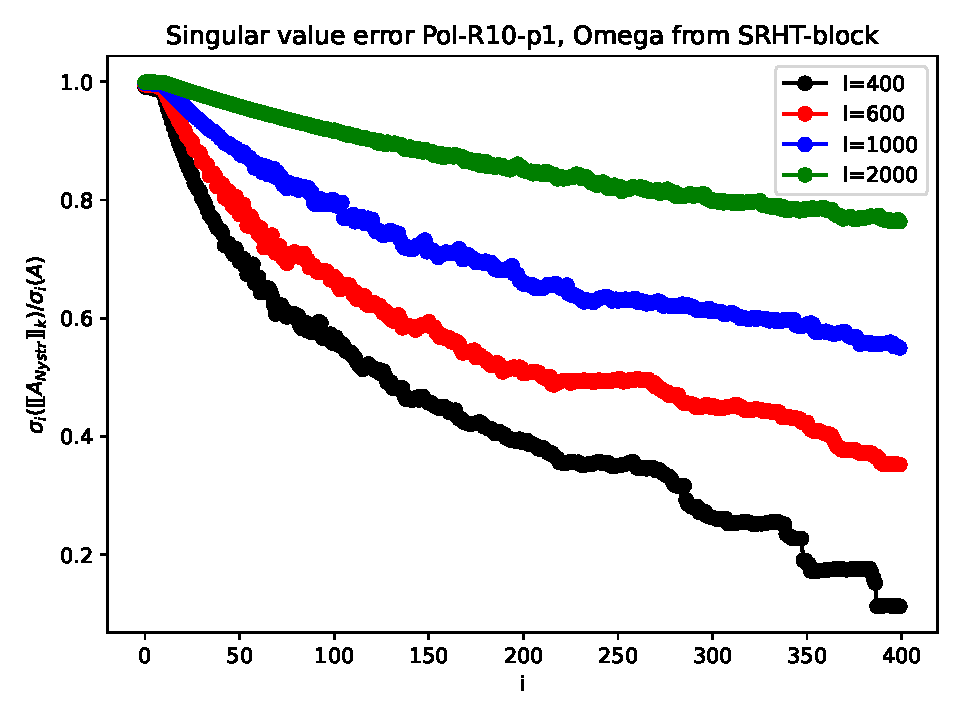
\includegraphics[width=\dimexpr\linewidth-20pt\relax]
        {../plots/singular_values/singular_values_Pol-R10-p1_SRHT-block.pdf}
    \makebox[20pt]{\raisebox{65pt}{\rotatebox[origin=c]{90}{Exponential decay}}}%
    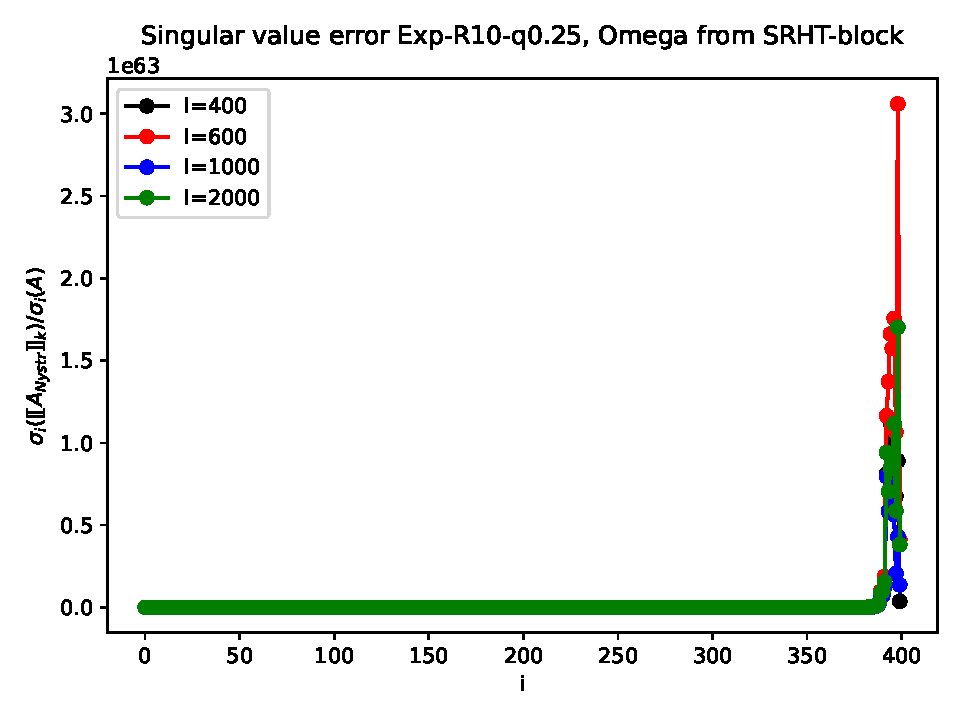
\includegraphics[width=\dimexpr\linewidth-20pt\relax]
        {../plots/singular_values/singular_values_Exp-R10-q0.25_SRHT-block.pdf}
    \caption{$\Omega$ created using BSRHT}
\end{subfigure}\hfill
\begin{subfigure}[t]{0.4\textwidth}
    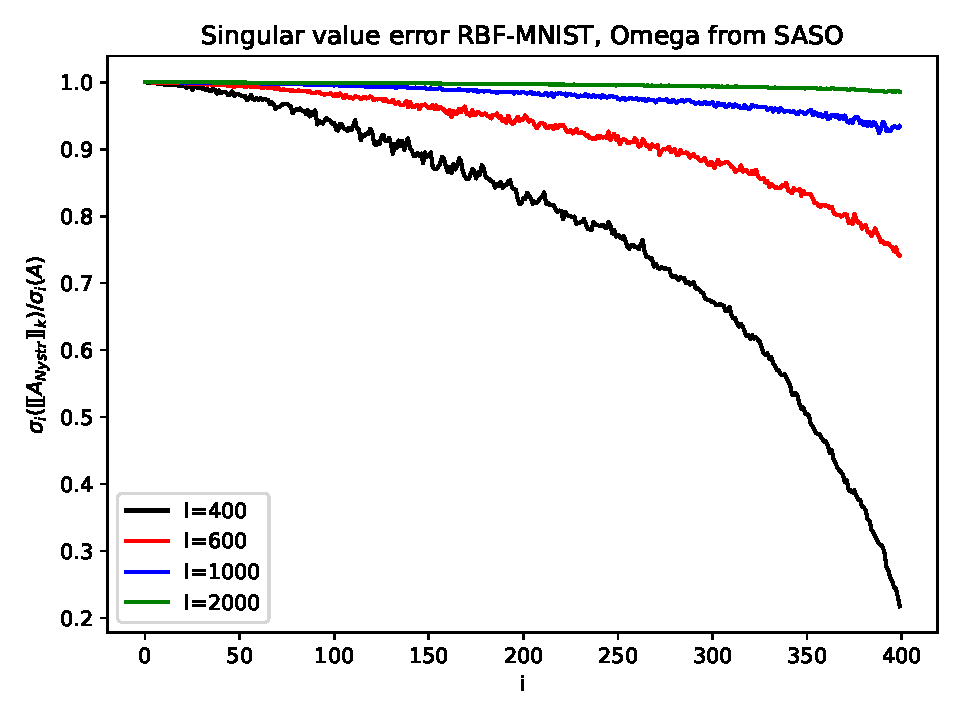
\includegraphics[width=\textwidth]
        {../plots/singular_values/singular_values_RBF-MNIST_SASO.pdf}
    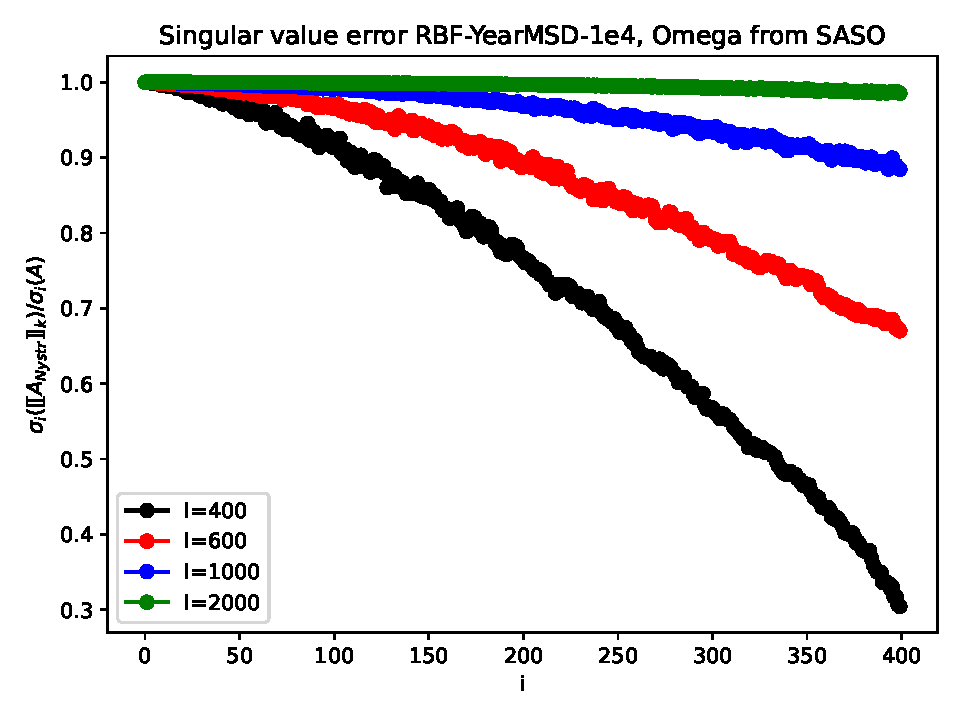
\includegraphics[width=\textwidth]
        {../plots/singular_values/singular_values_RBF-YearMSD-1e4_SASO.pdf}
    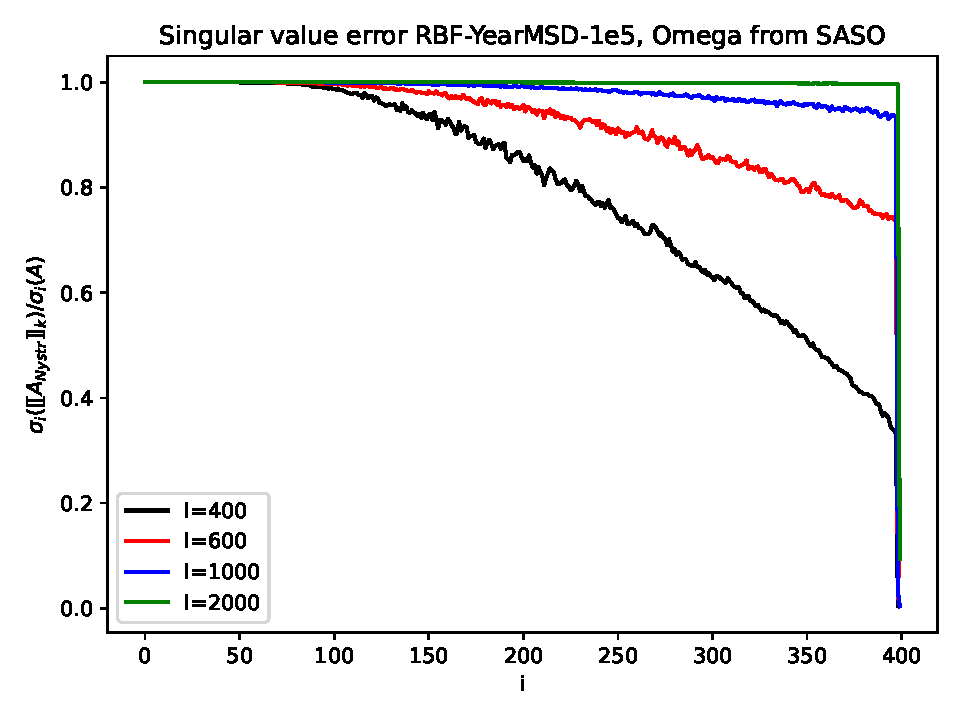
\includegraphics[width=\textwidth]
        {../plots/singular_values/singular_values_RBF-YearMSD-1e5_SASO.pdf}
    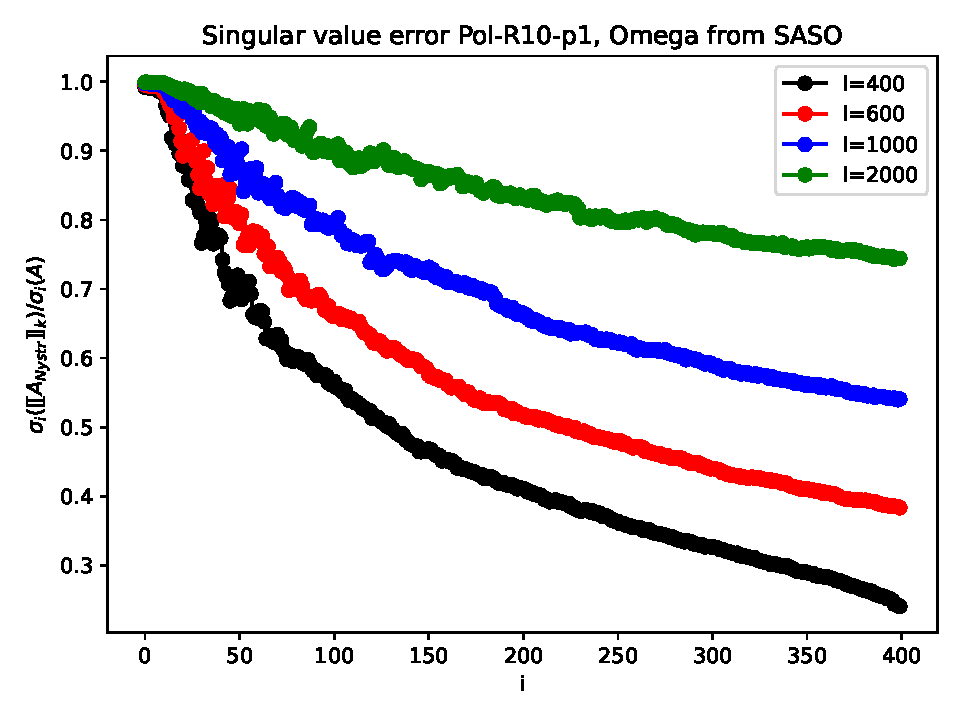
\includegraphics[width=\textwidth]
        {../plots/singular_values/singular_values_Pol-R10-p1_SASO.pdf}
    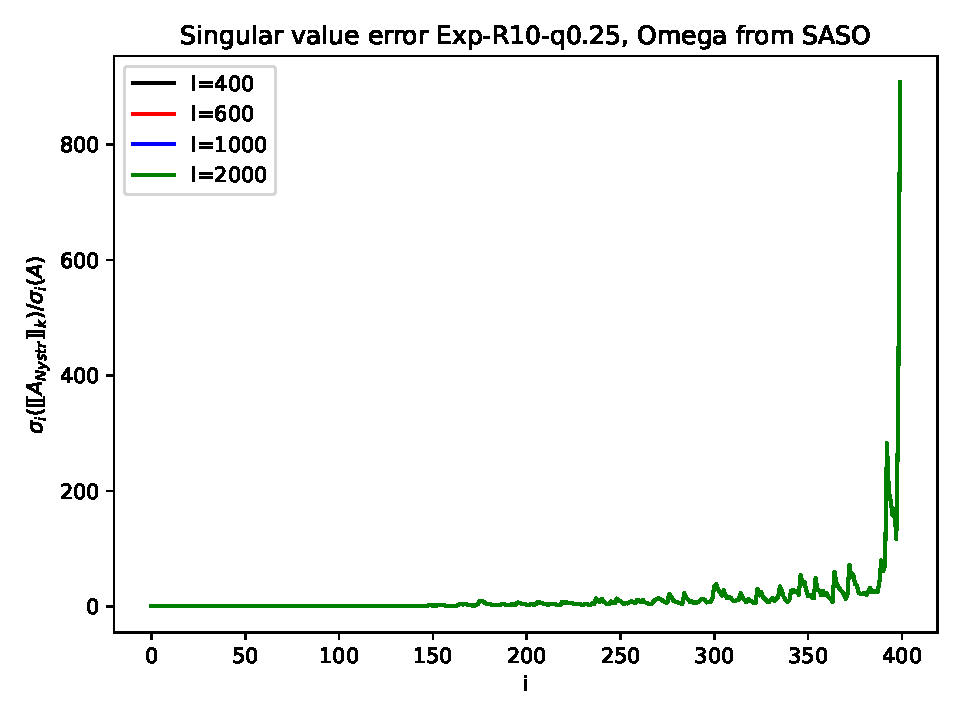
\includegraphics[width=\textwidth]
        {../plots/singular_values/singular_values_Exp-R10-q0.25_SASO.pdf}
    \caption{$\Omega$ created using SASO}
\end{subfigure}\hfill
\caption{Ratio of singular values for $k=400$ and different sketching dimensions
between Nyström approximation and original matrix.}
\label{fig:singularValueRatios}
\end{figure}

\section{Approximation of leading Singular Values}

In this section, we address the question of whether the leading $k$ singular
values of $A$ can be approximated using $[\![A_{Nystr}]\!]_k$. In particular, we
compare the largest $k$ singular values of $A$ and $[\![A_{Nystr}]\!]_k$
(ordered non-increasingly) and measure their ratio
\begin{align}
    \label{eq:singularValueError}
    \text{ratio}_{\sigma_i} := \frac{\sigma_i([\![A_{Nystr}]\!]_k)}{\sigma_i(A)}
    \quad \forall i \in \{1,...,k\}.
\end{align}

A ratio close to $1$ would lead to an error of the singular values close to $0$.
Figure \ref{fig:singularValueRatios} shows the ratio of singular values
$\text{ratio}_{\sigma_i}$ from equation (\ref{eq:singularValueError}) for both
sketching matrices and all datasets. We fixed the approximation rank to $k=400$,
once again computing the singular values via the SVD. Furthermore, we restrict
our investigations to the parallelized Nyström algorithm from Section
\ref{sec:parallel_nystrom} since we have seen in Section \ref{sec:num_stability}
that the sequential version (Algorithm \ref{algo:nyström}) produces similar
results.

For the 3 datasets using the RBF kernel, we see very similar results. Here we
find that (except the last few singular values for \texttt{YearMSD-1e5}) for
$l=400$ the ratio drops below $0.3$, whereas for $l=2000$ the first $400$
singular values are approximated with almost no loss. For $l=600$ and $l=1000$,
we find that the ratio stays above $0.7$ and $0.9$ respectively. That is, we
find a large difference between the sketching dimensions, with a worse ratio
(larger error) for the smaller singular values. For \texttt{Polynomial}, we see
similar behavior when altering the sketching dimension, but we are no longer
able to recreate the leading singular values for $l=2000$, so we do not expect
to be able to recreate the singular values for this dataset. For
\texttt{Exponential}, we see a good approximation for the first $\sim 70$
singular values, whereafter we see a steep decrease followed by a steep
increase. When comparing with the singular values of this dataset in Figure
\ref{fig:singularValue}, its singular values above $i=70$ are also significantly
below machine precision, so the error on the singular values is expected to be
low. \newline

Both sketching operators perform very similarly, with the only visible
difference for \texttt{Polynomial} for low sketching dimension, so this test
does not reveal which sketching matrix to choose. However, we do find that
choosing the sketching dimension $l$ as $5\cdot k$ looks to be a good and safe
rule of thumb. However, if you are working with these datasets, depending on the
usage, one would consider using $l=1000$ for the RBF datasets ($l$ being $2\cdot
k$ to $3\cdot k$ since $k=400$). Here $l=1000$ is chosen as the ratio of
approximated singular values is above 0.9 for all test cases and the
computational effort is significantly reduced when the sketching dimension is
halved compared to $l=2000$.

% Create a plot where we find the true first k singular values, and the k
% singular values of the Nyström approx. We can then subtract them to get k
% different error values, whereby we can easily see the minimum and maximum
% error (and how it evolves throughout k) of the approximation to the true. This
% can be done for all the different datasets, and for a single choice of l and
% k.

\section{Discussion and Conclusion}
To summarize, we found an efficient parallelization of the randomized Nyström
approximation which is stable and scales well w.r.t. the sketching dimension $l$
as well as the approximation rank $k$. We tested our approach on 5 different
datasets, real and synthetic to find and compare the numerical accuracy and
runtime performance of the algorithm. In particular, our parallel algorithm
produces similar numerical results as the sequential version but achieves a
speedup of up to 30\% on 4 processors. Furthermore, we compared the output
processed using the two sketching matrices SASO and SRHT (or BRSHT
respectively). Although one could expect SASO to provide lower overall runtimes
compared to SRHT, we observed this effect only partially and very limited in
practice. One might expect to see this effect more clearly with an
implementation exploiting sparsity. Regarding numerical stability, both
sketching operators produced similar results. Since there are stronger
theoretical approximation guarantees for BRSHT such as
(\ref{BRSHT:OSE_Condition}), BRSHT should be preferred when using our
implementation.\newline

For the numerical stability of the algorithm, we found a low relative error when
the decay of singular values was big enough, and found the Nyström approximation
to be good for datasets created using the RBF kernel with a properly chosen
$\sigma$ value. However, when the decay of singular values was big enough to
lead to a singular matrix, a change of algorithm was required for the
approximation, leading to a higher runtime, but still achieving a good
approximation.\newline

Approximating the leading $k$ singular values of $A$ using the Nyström
approximation is possible for fast decay of singular values, noting that the
ratio might be big if the singular values get very small. Judging from our
experiments, one should set $l$ between $2.5\cdot k$ and $5\cdot k$ to obtain a
decent approximation of the leading singular values, with the last few singular
values having a magnitude of $\sim 0.9$ of the original singular values.\newline

Finally, we want to point out some possible improvements for future work. First,
we considered only the randomized Nyström approximation which incorporates the
$Q$-factor of the $QR$ decomposition because it is sufficient for our relatively
small data dimension of $n = 2^{13}$ (see Section \ref{sec:rand_nystrom_alg}).
However, an investigation of the $Q$ vs. no-$Q$ version on a large-scale
distributed system with high-dimensional data, e.g. $n \geq 2^{16}$, would be
interesting. Second, all of our experiments were done on 4 processors on a
single machine. Therefore, we were unable to fully test the scaling capabilities
of our parallelization. Lastly, one could theoretically analyze the
computational cost of our parallel Nyström approximation in terms of
floating-point operations and communication cost and compare it with the found
numerical experiments.

\clearpage{}
% Moved bibliography above appendix
\printbibliography{} % print bibliography
\clearpage
\begin{appendices}
\section{Numerical Stability of Sequential Nyström}

\begin{figure}[!ht]
\centering
\hfill\begin{subfigure}[t]{\dimexpr0.35\textwidth+20pt\relax}
    \makebox[20pt]{\raisebox{65pt}{\rotatebox[origin=c]{90}{MNIST}}}%
    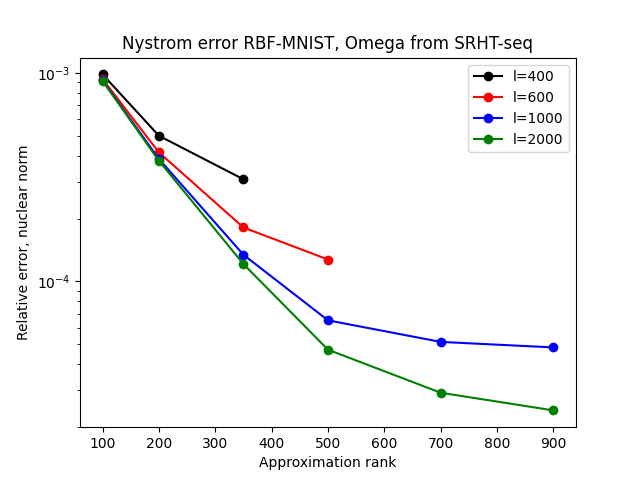
\includegraphics[width=\dimexpr\linewidth-20pt\relax]
        {../plots/relerror/relerror_RBF-MNIST_SRHT-seq.png}
    \makebox[20pt]{\raisebox{65pt}{\rotatebox[origin=c]{90}{YearMSD, $\sigma=10^4$}}}%
    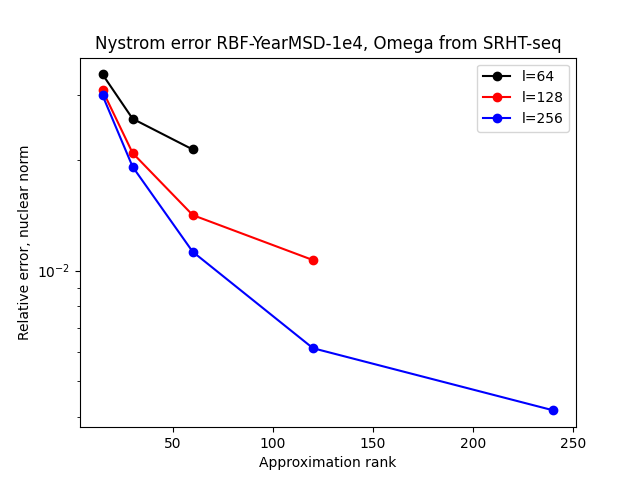
\includegraphics[width=\dimexpr\linewidth-20pt\relax]
        {../plots/relerror/relerror_RBF-YearMSD-1e4_SRHT-seq.png}
    \makebox[20pt]{\raisebox{65pt}{\rotatebox[origin=c]{90}{YearMSD, $\sigma=10^5$}}}%
    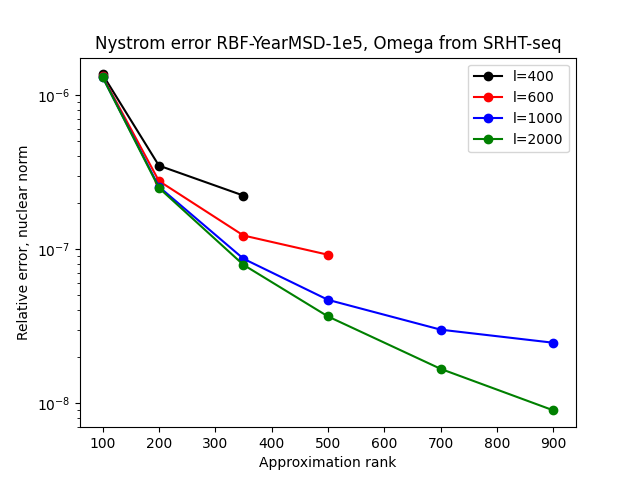
\includegraphics[width=\dimexpr\linewidth-20pt\relax]
        {../plots/relerror/relerror_RBF-YearMSD-1e5_SRHT-seq.png}
    \makebox[20pt]{\raisebox{65pt}{\rotatebox[origin=c]{90}{Polynomial decay}}}%
    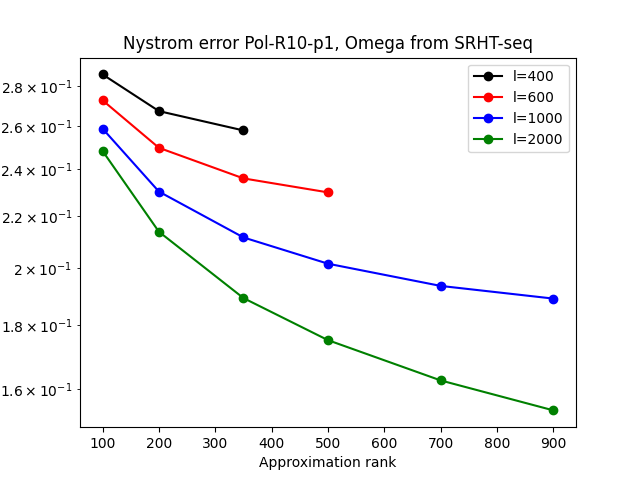
\includegraphics[width=\dimexpr\linewidth-20pt\relax]
        {../plots/relerror/relerror_Pol-R10-p1_SRHT-seq.png}
    \makebox[20pt]{\raisebox{65pt}{\rotatebox[origin=c]{90}{Exponential decay}}}%
    \includegraphics[width=\dimexpr\linewidth-20pt\relax]
        {../plots/relerror/relerror_Exp-R10-q0.25_SRHT-seq.png}
    \caption{$\Omega$ created using BSRHT}
\end{subfigure}\hfill
\begin{subfigure}[t]{0.35\textwidth}
    \includegraphics[width=\textwidth]
        {../plots/relerror/relerror_RBF-MNIST_SASO-seq.png}
    \includegraphics[width=\textwidth]
        {../plots/relerror/relerror_RBF-YearMSD-1e4_SASO-seq.png}
    \includegraphics[width=\textwidth]
        {../plots/relerror/relerror_RBF-YearMSD-1e5_SASO-seq.png}
    \includegraphics[width=\textwidth]
        {../plots/relerror/relerror_Pol-R10-p1_SASO-seq.png}
    \includegraphics[width=\textwidth]
        {../plots/relerror/relerror_Exp-R10-q0.25_SASO-seq.png}
    \caption{$\Omega$ created using SASO}
\end{subfigure}\hfill \caption{Relative error of the sequential version of the
randomized Nyström algorithm with different sketching matrices. Created for
comparison with Figure \ref{fig:RelError}, and is found to have very similar
(almost identical) performance.}
\label{fig:SequentialRelError}
\end{figure}
\end{appendices}

\end{document}
